\documentclass[a4paper]{article}
\usepackage{a4wide,amssymb,latexsym,multicol,array,hhline,fancyhdr}
\usepackage{vntex}
\usepackage{amsmath}
\usepackage{lastpage}
\usepackage{enumerate}
\usepackage{listings}
\usepackage{xcolor}
\usepackage{graphicx}
\usepackage{tabularx, caption}
\usepackage{multirow}
\usepackage{geometry}
\usepackage{setspace}
\usepackage{tikz}
\usepackage{indentfirst}
\usetikzlibrary{shapes, arrows, positioning, fit, calc, backgrounds}
\usepackage{float}
\usepackage[backend=bibtex,style=ieee]{biblatex}
\addbibresource{references.bib}
\usepackage[colorlinks]{hyperref}

\graphicspath{{images/}{figures/}}

% Màu và style code
\definecolor{codegray}{rgb}{0.5,0.5,0.5}
\definecolor{codepurple}{rgb}{0.6,0.2,0.6}
\definecolor{backcolor}{rgb}{0.95,0.95,0.95}
\def\labelitemi{--}

\lstdefinestyle{custom}{
    backgroundcolor=\color{backcolor},
    commentstyle=\color{codegray},
    keywordstyle=\color{blue},
    stringstyle=\color{codepurple},
    basicstyle=\ttfamily\small,
    breaklines=true,
    captionpos=b,
    keepspaces=true,
    numbers=left,
    numberstyle=\tiny\color{codegray},
    showstringspaces=false,
    tabsize=2
}
\lstset{style=custom}

% FORMATTING
\captionsetup[table]{name=Bảng}
\captionsetup[figure]{name=Hình}
\hypersetup{urlcolor=blue,linkcolor=black,citecolor=black,colorlinks=true}
\renewcommand{\arraystretch}{1.3}

% Ô đánh dấu phần chưa viết: \todo{Người phụ trách}{Nội dung cần viết}
\newcommand{\todo}[2]{%
  \par\noindent\fcolorbox{red}{yellow!25}{\parbox{\dimexpr\linewidth-2\fboxsep-2\fboxrule}{%
    \textbf{\color{red}TODO (#1):} #2}}\par\medskip}

% HEADER AND FOOTER
\setlength{\headheight}{40pt}
\pagestyle{fancy}
\fancyhead{}
\fancyhead[L]{
 \begin{tabular}{rl}
    \begin{picture}(25,15)(0,0)
    \put(0,-8){
\includegraphics[width=10mm, height=10mm]{hcmut.jpg}}
   \end{picture}&
    \begin{tabular}{l}
        \textbf{\bf \ttfamily Ho Chi Minh City University of Technology}\\
        \textbf{\bf \ttfamily Faculty of Computer Science and Engineering}
    \end{tabular}
 \end{tabular}
}
\fancyfoot{}
\fancyfoot[L]{\scriptsize \ttfamily Báo cáo Bài tập lớn Hệ quản trị Cơ sở dữ liệu - HK261}
\fancyfoot[R]{\scriptsize \ttfamily Trang {\thepage}/\pageref{LastPage}}
\renewcommand{\headrulewidth}{0.3pt}
\renewcommand{\footrulewidth}{0.3pt}

\setcounter{secnumdepth}{3}
\setcounter{tocdepth}{2}

\begin{document}

% BÌA BÁO CÁO
\begin{titlepage}
\begin{tikzpicture}[remember picture,overlay]
  \draw[line width=2pt]
    ($(current page.north west) + (1cm,-1cm)$) rectangle
    ($(current page.south east) + (-1cm,1cm)$);
\end{tikzpicture}
\begin{center}
{\Large \textbf{ĐẠI HỌC QUỐC GIA THÀNH PHỐ HỒ CHÍ MINH}}\\[0.3cm]
    {\Large \textbf{TRƯỜNG ĐẠI HỌC BÁCH KHOA}}\\[0.3cm]
    {\large \textbf{KHOA KHOA HỌC VÀ KỸ THUẬT MÁY TÍNH}}\\[1cm]
\end{center}

\vspace{0.5cm}

\begin{figure}[h!]
\begin{center}

\includegraphics[width=4cm]{hcmut.jpg}
\end{center}
\end{figure}
\vspace{0.5cm}
\begin{flushleft}
    \large \textbf{BÀI TẬP LỚN HỆ QUẢN TRỊ CƠ SỞ DỮ LIỆU} \\
    \rule{\linewidth}{0.3pt} \\
    \begin{center}
        \huge \textbf{Hệ thống Quản lý Phòng khám Đa khoa kết hợp SQL Server và Cassandra} \\
        \rule{\linewidth}{0.3pt}
    \end{center}
\end{flushleft}

\begin{table}[h]
\centering
\renewcommand{\arraystretch}{1.7}
\setlength{\tabcolsep}{10pt}
\begin{tabular}{ll}
\textbf{Giảng viên hướng dẫn:} & \colorbox{yellow!40}{TODO: tên GVHD} \\
\textbf{Lớp:} & L01 \\
\textbf{Sinh viên thực hiện:} & Nguyễn Thái Vũ Hoàng - 2311063 \\
& \colorbox{yellow!40}{TODO: họ tên Dương - MSSV} \\
\textbf{Mã nguồn (GitHub):} & \href{https://github.com/Conductor15/healthcare-dbms}{\color{blue}\underline{Truy cập tại đây}} \\
\end{tabular}
\end{table}

\begin{center}
{\footnotesize TP. HỒ CHÍ MINH, THÁNG 11 NĂM 2026}
\end{center}
\end{titlepage}

% MỤC LỤC
\tableofcontents
\newpage

\section{Giới thiệu}

\subsection{Bối cảnh}
Một phòng khám đa khoa cần quản lý hai loại dữ liệu có tính chất trái ngược nhau:
\begin{itemize}
    \item \textbf{Dữ liệu nghiệp vụ lâm sàng và tài chính}: hồ sơ bệnh nhân, bác sĩ, lịch hẹn, lượt khám, đơn thuốc, tồn kho, hoá đơn. Dữ liệu có quan hệ chặt, được nhiều người sửa đồng thời (lễ tân, bác sĩ, thu ngân). Đây là dữ liệu có giá trị pháp lý: không được mất, không được sai lệch.
    \item \textbf{Dữ liệu thiết bị và hệ thống}: chỉ số sinh hiệu do máy đo gửi liên tục (nhịp tim, huyết áp, SpO$_2$, nhiệt độ) và nhật ký truy cập. Dữ liệu chỉ ghi thêm, khối lượng lớn, đọc theo mẫu cố định (theo bệnh nhân và thời gian), cần ghi được kể cả khi một máy chủ gặp sự cố.
\end{itemize}

Hai nhóm dữ liệu trên đặt ra các yêu cầu khác nhau về tính nhất quán, khả năng mở rộng và tính sẵn sàng, nên khó có một hệ quản trị đáp ứng tốt cả hai. Đề tài khảo sát Microsoft SQL Server (hệ quản trị quan hệ) và Apache Cassandra (hệ quản trị NoSQL dạng wide-column) qua sáu chủ đề của môn học, so sánh kết quả thực nghiệm trên từng chủ đề để xác định vai trò phù hợp của mỗi hệ quản trị đối với từng nhóm dữ liệu. Kết quả này được hiện thực trong một ứng dụng sử dụng đồng thời cả hai hệ quản trị theo mô hình \textit{polyglot persistence}.

\subsection{Mục tiêu và phạm vi}

\begin{table}[H]
\centering
\caption{Mục tiêu và phạm vi thực hiện}
\begin{tabularx}{\linewidth}{|p{3.6cm}|X|}
\hline
\textbf{Mục tiêu} & \textbf{Phạm vi thực hiện} \\ \hline
So sánh 2 DBMS theo các chủ đề của môn học & Cả \textbf{6/6 chủ đề} (đề yêu cầu tối thiểu 2 với nhóm 2 người): lưu trữ, chỉ mục, xử lý truy vấn, giao dịch, điều khiển đồng thời, sao lưu và phục hồi. Mỗi chủ đề có kịch bản trên \textbf{cả hai} DBMS, số đo, bảng so sánh và kết luận cho bối cảnh phòng khám. \\ \hline
Xây dựng ứng dụng & Ứng dụng web n-tier với \textbf{9 chức năng} (đề yêu cầu 4), đủ \textbf{8 loại truy vấn/cập nhật}, dùng \textbf{cả hai} DBMS theo mô hình \textit{polyglot persistence}. \\ \hline
Đưa kết quả nghiên cứu vào ứng dụng & Trang \textbf{DB Lab} chạy các thí nghiệm ngay trong ứng dụng; các kỹ thuật rút ra (khoá chống đặt trùng lịch, transaction kê đơn, logged batch, point-in-time restore) được dùng trong chức năng thật. \\ \hline
\end{tabularx}
\end{table}

\subsection{Phân công tổng quan}

\begin{table}[H]
\centering
\caption{Phân công tổng quan}
\begin{tabularx}{\linewidth}{|p{2.4cm}|X|X|p{3cm}|}
\hline
\textbf{Thành viên} & \textbf{Chủ đề DBMS} & \textbf{Chức năng ứng dụng} & \textbf{Khác} \\ \hline
Hoàng (trưởng nhóm) & iv. Transaction, v. Concurrency control, vi. Backup \& recovery & FR3 Lịch hẹn, FR4 Khám \& kê đơn, FR6 Chi tiết lượt khám, FR9 Sinh hiệu (Cassandra), nhật ký truy cập, DB Lab iv--vi & Hạ tầng, quy trình làm việc, kiểm thử \\ \hline
Dương & i. Data storage \& management, ii. Indexing, iii. Query processing & FR1 Bệnh nhân, FR2 Bác sĩ, FR5 Tìm kiếm, FR7 Thống kê, FR8 Truy vấn nâng cao, DB Lab i--iii & Mô hình dữ liệu Cassandra, bộ sinh dữ liệu lớn \\ \hline
\end{tabularx}
\end{table}

Chi tiết đóng góp được trình bày ở Mục~\ref{sec:teamwork}.

\subsection{Cấu trúc báo cáo}
Mục~\ref{sec:background} giới thiệu hai DBMS và môi trường thực nghiệm. Mục~\ref{sec:demo} trình bày thực nghiệm và so sánh cho 6 chủ đề. Mục~\ref{sec:app} mô tả ứng dụng: yêu cầu, kiến trúc, thiết kế dữ liệu, hiện thực và trang DB Lab. Mục~\ref{sec:teamwork} báo cáo cách làm việc nhóm. Mục~\ref{sec:conclusion} kết luận và tự đánh giá theo tiêu chí chấm điểm.

\section{Tổng quan hai DBMS và môi trường thực nghiệm}
\label{sec:background}

\subsection{Microsoft SQL Server 2022}

\subsubsection{Kiến trúc tổng quan}
SQL Server là hệ quản trị cơ sở dữ liệu quan hệ của Microsoft, dùng ngôn ngữ T-SQL. Một instance SQL Server gồm hai thành phần chính~\cite{silberschatz}:
\begin{itemize}
    \item \textbf{Relational Engine (Query Processor)}: phân tích câu lệnh, tối ưu hoá dựa trên chi phí (cost-based optimizer) với thống kê dữ liệu, sinh và lưu kế hoạch thực thi (plan cache), điều phối việc thực thi.
    \item \textbf{Storage Engine}: quản lý truy cập dữ liệu (heap, B$^+$-tree), bộ đệm (buffer pool), khoá (lock manager), phiên bản dòng (version store) và transaction log.
\end{itemize}
Bên dưới là lớp SQLOS lo lập lịch luồng, quản lý bộ nhớ và phát hiện deadlock.

\subsubsection{Tổ chức lưu trữ}
Mỗi cơ sở dữ liệu có ít nhất một file dữ liệu (\texttt{.mdf}, \texttt{.ndf}) và một file log (\texttt{.ldf}). File dữ liệu được chia thành các \textbf{trang 8 KB}; 8 trang liên tiếp tạo thành một \textbf{extent 64 KB}~\cite{mssql-pages}. Bảng được lưu dưới dạng heap hoặc clustered index (B$^+$-tree theo khoá clustered); nonclustered index là các B$^+$-tree riêng trỏ về dòng dữ liệu. Chi tiết lưu trữ và chỉ mục được phân tích trong Mục~\ref{sec:storage} và Mục~\ref{sec:indexing}.

File log ghi tuần tự, chia thành các \textit{virtual log file}. Mỗi thay đổi dữ liệu được ghi vào log trước (\textit{write-ahead logging}) rồi mới sửa trang trong buffer pool; trang bẩn được ghi xuống đĩa sau, ở checkpoint hoặc bởi lazy writer~\cite{mssql-txlog}. Cơ chế này là nền tảng cho transaction (Mục~\ref{sec:transaction}) và phục hồi (Mục~\ref{sec:backup}).

\subsubsection{Giao dịch, đồng thời và phục hồi}
\begin{itemize}
    \item \textbf{Transaction} đầy đủ ACID trên nhiều câu lệnh, nhiều bảng; hỗ trợ savepoint và xử lý lỗi \texttt{TRY\ldots CATCH}.
    \item \textbf{Điều khiển đồng thời} kết hợp hai cơ chế: khoá nhiều mức độ (KEY, PAGE, OBJECT) với leo thang khoá, và \textit{row versioning} (SNAPSHOT, READ COMMITTED SNAPSHOT) lưu phiên bản cũ trong tempdb~\cite{mssql-locking}. Có 4 mức cô lập theo chuẩn ANSI cộng mức SNAPSHOT.
    \item \textbf{Phục hồi}: crash recovery tự động theo họ thuật toán ARIES~\cite{aries}; ba \textit{recovery model} (SIMPLE, BULK\_LOGGED, FULL) quyết định log được giữ bao lâu và có khôi phục tới một thời điểm được hay không~\cite{mssql-recovery}. SQL Server Agent lập lịch các job sao lưu.
\end{itemize}

\subsubsection{Các tính năng được dùng trong đề tài}

\begin{table}[H]
\centering
\caption{Tính năng SQL Server được sử dụng}
\label{tab:mssql-features}
\begin{tabularx}{\linewidth}{|p{4.6cm}|X|}
\hline
\textbf{Tính năng} & \textbf{Dùng ở đâu} \\ \hline
Transaction, \texttt{XACT\_ABORT}, savepoint & Thí nghiệm Mục~\ref{sec:transaction}; đặt lịch (FR3), khám bệnh (FR4) \\ \hline
Mức cô lập, table hint \texttt{UPDLOCK}, \texttt{HOLDLOCK} & Thí nghiệm Mục~\ref{sec:concurrency}; chống đặt trùng lịch (FR3) \\ \hline
Filtered UNIQUE index, \texttt{CHECK} constraint & Lớp chặn cuối cho lịch hẹn; tồn kho không âm \\ \hline
\texttt{UPDATE \ldots{} OUTPUT} & Trừ tồn kho và lấy giá thuốc trong một câu (FR4) \\ \hline
DMV \texttt{sys.dm\_tran\_locks}, \texttt{fn\_dblog} & Quan sát khoá, deadlock, bản ghi log \\ \hline
\texttt{BACKUP}/\texttt{RESTORE \ldots{} STOPAT}, SQL Server Agent & Thí nghiệm Mục~\ref{sec:backup}; DB Lab \\ \hline
\end{tabularx}
\end{table}

\subsection{Apache Cassandra 5.0}
\todo{Dương}{Kiến trúc phân tán (ring, partitioner, replication), mô hình wide-column, đường ghi (commit log $\rightarrow$ memtable $\rightarrow$ SSTable), thiết kế theo truy vấn.}

\subsection{Môi trường thực nghiệm}
Toàn bộ thực nghiệm và ứng dụng chạy trên Docker Compose, nên cả hai thành viên có môi trường giống hệt nhau. Lệnh \texttt{npm run db:init} tạo lại cơ sở dữ liệu từ các script trong thư mục \texttt{database/}.

\begin{table}[H]
\centering
\caption{Cấu hình môi trường thực nghiệm}
\label{tab:env}
\begin{tabularx}{\linewidth}{|p{3.5cm}|X|}
\hline
\textbf{Thành phần} & \textbf{Cấu hình} \\ \hline
Máy thực nghiệm & AMD Ryzen 7 6800H (8 nhân, 16 luồng), RAM 32 GB, SSD NVMe Samsung 512 GB, Windows 11 \\ \hline
Docker & Docker Desktop 29.6 trên WSL2, cấp 16 CPU và 16 GB RAM \\ \hline
SQL Server & Image \texttt{mssql/server:2022-latest}, bản Developer, bật SQL Server Agent, 1 container \\ \hline
Cassandra & Image \texttt{cassandra:5.0}, heap 1 GB, datacenter \texttt{dc1}. Mặc định 1 node; bật thêm 2 node (\texttt{-{}-profile cluster}) cho các thí nghiệm consistency và replication \\ \hline
Ứng dụng & Node.js 24, Express 5; React 19, Ant Design 6, Vite 7 \\ \hline
Bộ đo hiệu năng & \texttt{demos/\_common/bench.js}: chạy truy vấn $N$ lần trên 2 DB, xuất CSV (min/avg/p50/p95, logical reads, throughput song song) \\ \hline
\end{tabularx}
\end{table}

Các thí nghiệm ở Mục~\ref{sec:transaction}--\ref{sec:backup} dùng dữ liệu mẫu do \texttt{npm run db:init} tạo ra, cộng với dữ liệu do chính script thí nghiệm sinh thêm (ví dụ 20\,000 dòng cho thí nghiệm log, 10\,000 dòng cho leo thang khoá).

\todo{Dương}{Mô tả bộ dữ liệu lớn (S1.4): số bệnh nhân, lượt khám, bản ghi sinh hiệu ở từng mức scale.}

\section{Thực nghiệm và so sánh hai DBMS}
\label{sec:demo}

Mỗi chủ đề được trình bày theo cùng một trình tự: cơ sở lý thuyết, thiết lập thí nghiệm, kết quả, thảo luận và kết luận cho bối cảnh phòng khám. Script, số liệu và output đầy đủ nằm trong thư mục \texttt{demos/} của mã nguồn.

%==================================================================
\subsection{Data storage \& management}
\label{sec:storage}
\todo{Dương}{Chủ đề i (T1): lý thuyết, kịch bản, kết quả trên SQL Server và Cassandra, so sánh, kết luận cho phòng khám.}

%==================================================================
\subsection{Indexing}
\label{sec:indexing}
\todo{Dương}{Chủ đề ii (T2, topic chính của Dương).}

%==================================================================
\subsection{Query processing}
\label{sec:query}
\todo{Dương}{Chủ đề iii (T3).}

%==================================================================
\subsection{Transaction}
\label{sec:transaction}

\subsubsection{Cơ sở lý thuyết}
Một transaction là một đơn vị công việc thoả \textbf{ACID}~\cite{silberschatz}: \textit{Atomicity} (tất cả hoặc không gì cả), \textit{Consistency} (đưa CSDL từ trạng thái hợp lệ sang trạng thái hợp lệ), \textit{Isolation} (các transaction đồng thời không thấy trạng thái dở dang của nhau), \textit{Durability} (đã commit thì không mất kể cả khi sập máy).

\textbf{SQL Server} hỗ trợ transaction đầy đủ trên nhiều câu lệnh và nhiều bảng (\texttt{BEGIN TRAN \ldots{} COMMIT/ROLLBACK}, savepoint \texttt{SAVE TRAN}, \texttt{TRY\ldots CATCH}). Durability dựa trên \textit{write-ahead logging}: bản ghi log (ảnh trước/sau của dữ liệu) được ghi xuống file \texttt{.ldf} trước khi \texttt{COMMIT} trả về; trang dữ liệu được ghi sau, ở checkpoint~\cite{mssql-txlog}. Ba chế độ: autocommit (mặc định), implicit, explicit.

\textbf{Cassandra} không có transaction nhiều partition. Mỗi lần ghi trong \textit{một} partition là atomic và isolated. \texttt{BATCH} dạng \textit{logged} đảm bảo mọi câu trong batch \textit{cuối cùng} đều được áp dụng (ghi vào batchlog trước), nhưng \textbf{không có isolation} và không có \texttt{ROLLBACK}~\cite{cassandra-docs}. \textit{Lightweight transaction} (LWT: \texttt{IF NOT EXISTS}, \texttt{IF <điều kiện>}) dùng giao thức Paxos~\cite{paxos} để compare-and-set tuyến tính hoá trên \textbf{một} partition. Cột thường không hỗ trợ phép toán đọc-sửa-ghi như \texttt{stock = stock - 10}.

\subsubsection{Thiết lập thí nghiệm}
Nghiệp vụ dùng xuyên suốt là \textbf{``khám bệnh''}: một lượt khám ghi 5 bảng (\texttt{visits}, \texttt{prescriptions}, \texttt{prescription\_items}, trừ \texttt{medicines.stock\_quantity}, \texttt{invoices}). Ràng buộc \texttt{CK\_medicines\_stock CHECK (stock\_quantity >= 0)} biến việc kê vượt tồn kho thành lỗi thật. Trên Cassandra, cùng nghiệp vụ được mô hình bằng các bảng phi chuẩn hoá trong keyspace \texttt{tx\_demo}.

\subsubsection{Kết quả}

\begin{table}[H]
\centering
\caption{Các kịch bản transaction trên hai DBMS}
\small
\begin{tabularx}{\linewidth}{|c|p{2.8cm}|X|X|}
\hline
\textbf{\#} & \textbf{Kịch bản} & \textbf{SQL Server} & \textbf{Cassandra} \\ \hline
1 & Lỗi ở bước 4/5 của quy trình khám & \texttt{XACT\_STATE() = -1} $\rightarrow$ ROLLBACK; số dòng 4 bảng và tồn kho \textbf{trước = sau} & Câu 1 đã được ghi vĩnh viễn; khi ứng dụng dừng, CSDL còn lại \textbf{lượt khám không có hoá đơn}; \texttt{ROLLBACK} $\rightarrow$ \texttt{SyntaxException} \\ \hline
2 & \texttt{XACT\_ABORT OFF} (mặc định) & Lỗi chỉ huỷ \textbf{một câu}, transaction vẫn mở, \texttt{COMMIT} lưu \textbf{nửa transaction} (Paracetamol bị trừ, Salbutamol không). \texttt{ON} $\rightarrow$ rollback toàn bộ & -- \\ \hline
3 & Savepoint & Thuốc thứ 3 hết hàng $\rightarrow$ \texttt{ROLLBACK TRAN sp} chỉ bỏ thuốc 3, giữ thuốc 1--2. Chỉ dùng được khi \texttt{XACT\_ABORT OFF} & -- \\ \hline
4 & Batch nhiều bảng & -- & Áp dụng đủ 3 bảng; batch có 1 câu sai kiểu bị từ chối toàn bộ; batch có điều kiện \textbf{không được} trải nhiều bảng \\ \hline
5 & LWT & -- & \texttt{IF NOT EXISTS} lần 2: \texttt{[applied]=False}; \texttt{IF stock = 100}: lệnh của client thứ 2 không được áp dụng \\ \hline
6 & Log của 1 transaction (\texttt{fn\_dblog}) & \texttt{LOP\_BEGIN\_XACT} $\rightarrow$ \texttt{LOP\_MODIFY\_COLUMNS} $\times 2$ $\rightarrow$ \texttt{LOP\_COMMIT\_XACT} & -- \\ \hline
7 & Crash (\texttt{kill -9}) & Xem Mục~\ref{sec:backup}: dữ liệu đã commit được REDO, chưa commit bị UNDO & Commit log replay \\ \hline
\end{tabularx}
\end{table}

\textbf{Torn read}: 1 writer cập nhật 2 dòng \textit{trong cùng một} transaction/batch, 4 reader đọc liên tục trong 4 giây và đếm số lần thấy 2 dòng lệch phiên bản (Bảng~\ref{tab:torn-read}).

\begin{table}[H]
\centering
\caption{Tỉ lệ torn read theo DBMS và mức đọc}
\label{tab:torn-read}
\begin{tabular}{|l|l|r|r|}
\hline
\textbf{DBMS} & \textbf{Cách ghi / mức đọc} & \textbf{Lượt đọc} & \textbf{Torn read} \\ \hline
SQL Server & READ UNCOMMITTED & 10\,166 & 0.51\% \\ \hline
SQL Server & READ COMMITTED (mặc định) & 3\,360 & \textbf{0.15\%} \\ \hline
SQL Server & REPEATABLE READ & 3\,365 & 0 \\ \hline
SQL Server & SNAPSHOT & 11\,165 & 0 \\ \hline
Cassandra & LOGGED batch & 13\,351 & \textbf{5.22\%} \\ \hline
Cassandra & UNLOGGED batch & 18\,526 & 9.75\% \\ \hline
\end{tabular}
\end{table}

\begin{table}[H]
\centering
\caption{Chi phí ghi 2000 dòng}
\label{tab:tx-cost}
\begin{tabular}{|l|l|r|}
\hline
\textbf{DBMS} & \textbf{Cách ghi} & \textbf{Dòng/s} \\ \hline
SQL Server & Autocommit, 1 client (2000 lần flush log) & 152 \\ \hline
SQL Server & 1 transaction cho 2000 dòng & 1\,169 ($\times 7.7$) \\ \hline
SQL Server & Autocommit, 16 client & 1\,194 \\ \hline
Cassandra & INSERT đơn, 1 client / 16 client & 1\,095 / 15\,488 \\ \hline
Cassandra & UNLOGGED batch 50 dòng cùng partition & 30\,200 \\ \hline
Cassandra & LWT \texttt{IF NOT EXISTS} & 581 (chậm $\times 1.9$) \\ \hline
\end{tabular}
\end{table}

\subsubsection{Thảo luận}
\begin{itemize}
    \item Batch của Cassandra là \textbf{atomic nhưng không isolated}: 5\% số lần đọc thấy trạng thái chưa hoàn tất của batch.
    \item READ COMMITTED của SQL Server cũng không đảm bảo đọc nhất quán \textit{nhiều dòng}, vì khoá S nhả sau từng dòng. Muốn nhất quán thì cần REPEATABLE READ (giữ khoá) hoặc SNAPSHOT (đọc phiên bản). SNAPSHOT vừa đúng vừa không chặn writer, nên đọc được nhiều gấp 3.3 lần.
    \item Chi phí chính của transaction SQL Server là flush log lúc commit; gom thao tác vào một transaction tăng tốc 7.7 lần.
    \item Cassandra đạt throughput ghi cao do không duy trì transaction. Khi cần đảm bảo tính đúng đắn bằng LWT, chi phí tăng do các vòng trao đổi của giao thức Paxos.
\end{itemize}

\subsubsection{Kết luận cho bối cảnh phòng khám}
Khám bệnh, kê đơn, trừ kho, lập hoá đơn, đặt lịch là các nghiệp vụ \textbf{bắt buộc atomic trên nhiều bảng}, nên dùng SQL Server. Ứng dụng chạy chúng trong \texttt{withTransaction()} (luôn rollback khi có lỗi, tránh trường hợp commit một phần như kịch bản 2). Dữ liệu sinh hiệu chỉ cần atomic trong một lần đo, và ứng dụng dùng \textit{logged batch} để ghi 3 bảng phi chuẩn hoá của một lần đo trên Cassandra.

%==================================================================
\subsection{Concurrency control}
\label{sec:concurrency}

\subsubsection{Cơ sở lý thuyết}
\textbf{SQL Server} mặc định dùng \textit{pessimistic locking}~\cite{mssql-locking}: khoá chia sẻ (S), cập nhật (U), độc quyền (X) cùng khoá ý định (IS/IX/SIX) theo cây tài nguyên KEY $\rightarrow$ PAGE $\rightarrow$ OBJECT. Khi một câu lệnh giữ quá nhiều khoá ($\sim$5000) thì \textit{leo thang} thành khoá cả bảng. Mức cô lập quyết định khoá S được giữ bao lâu: READ UNCOMMITTED (không lấy khoá S), READ COMMITTED (nhả sau mỗi dòng), REPEATABLE READ (giữ tới cuối transaction), SERIALIZABLE (giữ thêm khoá khoảng). Ngoài ra có hai mức dựa trên \textbf{MVCC} (version store trong tempdb): SNAPSHOT và READ COMMITTED SNAPSHOT. Deadlock được một tiến trình nền phát hiện, nó chọn một \textit{victim} để huỷ (lỗi 1205).

\textbf{Cassandra} không dùng khoá. Mỗi ô dữ liệu mang \textit{write timestamp} và giá trị có timestamp lớn nhất thắng (\textit{last-write-wins}). Nhất quán giữa các bản sao là \textbf{tunable}~\cite{cassandra-docs}: mỗi câu lệnh chọn consistency level (ONE, QUORUM, ALL). Đọc và ghi nhất quán mạnh khi $R + W > RF$. Muốn compare-and-set thì dùng LWT (Paxos) trên một partition.

\subsubsection{Kết quả}

\textbf{Thí nghiệm 1: hiện tượng $\times$ mức cô lập} (SQL Server, 2 phiên xen kẽ tất định, lock timeout 1.5 s). Dấu $\times$ nghĩa là hiện tượng xảy ra, $\checkmark$ nghĩa là được ngăn chặn kèm cơ chế ngăn chặn.

\begin{table}[H]
\centering
\caption{Hiện tượng bất thường theo mức cô lập trên SQL Server}
\label{tab:isolation}
\small
\begin{tabularx}{\linewidth}{|p{3.2cm}|X|X|X|X|X|}
\hline
\textbf{Hiện tượng} & \textbf{READ UNCOMMITTED} & \textbf{READ COMMITTED} & \textbf{REPEATABLE READ} & \textbf{SERIALIZABLE} & \textbf{SNAPSHOT} \\ \hline
Dirty read & $\times$ & $\checkmark$ khoá & $\checkmark$ khoá & $\checkmark$ khoá & $\checkmark$ phiên bản \\ \hline
Non-repeatable read & $\times$ & $\times$ & $\checkmark$ khoá & $\checkmark$ khoá & $\checkmark$ phiên bản \\ \hline
Phantom read & $\times$ & $\times$ & $\times$ & $\checkmark$ khoá khoảng & $\checkmark$ phiên bản \\ \hline
Lost update (đọc rồi ghi) & $\times$ & $\times$ & $\checkmark$ chặn $\rightarrow$ thử lại & $\checkmark$ chặn $\rightarrow$ thử lại & $\checkmark$ xung đột 3960 \\ \hline
Lost update (\texttt{qty = qty - 10}) & $\checkmark$ & $\checkmark$ & $\checkmark$ & $\checkmark$ & $\checkmark$ \\ \hline
\end{tabularx}
\end{table}

Kết quả khớp hoàn toàn bảng lý thuyết (25/25 ô) và cho thấy ba cơ chế: khoá, đa phiên bản, phát hiện xung đột.

\textbf{Thí nghiệm 2: 50 bệnh nhân đặt cùng một khung giờ} (chức năng FR3).

\begin{table}[H]
\centering
\caption{Double-booking: 50 yêu cầu đồng thời cho cùng một khung giờ}
\label{tab:double-booking}
\begin{tabular}{|l|c|c|}
\hline
\textbf{Cách làm} & \textbf{Báo thành công} & \textbf{Bản ghi lưu} \\ \hline
SQL Server, đọc \texttt{is\_booked} rồi ghi, không khoá & 50 & \textbf{50} \\ \hline
SQL Server, transaction + \texttt{WITH (UPDLOCK, HOLDLOCK)} & 1 & 1 \\ \hline
SQL Server, chỉ UNIQUE index & 1 (49 lỗi 2627) & 1 \\ \hline
Cassandra, SELECT rồi INSERT & 50 & 1 (\textbf{ghi đè, không báo lỗi}) \\ \hline
Cassandra, \texttt{INSERT \ldots{} IF NOT EXISTS} & 1 & 1 \\ \hline
\end{tabular}
\end{table}

\textbf{Thí nghiệm 3: khoá và leo thang khoá.} UPDATE 100 dòng giữ 100 khoá \texttt{KEY X} và khoá ý định IX ở PAGE/OBJECT. UPDATE 10\,000 dòng thì leo thang thành \texttt{OBJECT X}. Tắt leo thang thì giữ 10\,000 khoá \texttt{KEY X}.

\textbf{Thí nghiệm 4: deadlock.} T1 giữ thuốc 1 chờ thuốc 2, T2 ngược lại; \texttt{sys.dm\_tran\_locks} cho thấy khoá \texttt{KEY X} ở trạng thái WAIT. SQL Server phát hiện sau khoảng 1.2 s, chọn một victim (1205); victim thử lại thì tồn kho cuối đúng.

\textbf{Thí nghiệm 5: last-write-wins.} Bản đo $t=5$ thắng bản $t=3$ dù đến trước. Bản retry cũ ($t=1$) đến sau \textbf{bị bỏ qua không báo lỗi}. Xung đột được giải quyết theo từng ô (2 client sửa 2 cột khác nhau đều giữ được).

\textbf{Thí nghiệm 6: tunable consistency} (3 node, $RF = 3$, tắt hinted handoff). Kịch bản: node 3 ngừng hoạt động trong lúc hệ thống ghi thông tin dị ứng \textit{penicillin} của một bệnh nhân.

\begin{table}[H]
\centering
\caption{Tunable consistency trên cluster 3 node}
\label{tab:consistency}
\begin{tabularx}{\linewidth}{|X|c|X|}
\hline
\textbf{Bước} & \textbf{CL} & \textbf{Kết quả} \\ \hline
Ghi khi node 3 ngừng hoạt động & ALL & Unavailable (cần 3, còn 2) \\ \hline
Ghi khi node 3 ngừng hoạt động & QUORUM & OK \\ \hline
Node 3 hoạt động lại, đọc $\times 5$ qua node 3 & ONE & \texttt{penicillin} $\times 2$, \texttt{none} $\times 3$: \textbf{bỏ sót dị ứng 3/5 lần} \\ \hline
Đọc qua node 3 & QUORUM & \texttt{penicillin} ($R + W = 4 > 3$), read repair sửa node 3 \\ \hline
\end{tabularx}
\end{table}

\subsubsection{Thảo luận và kết luận cho bối cảnh phòng khám}
\begin{itemize}
    \item Tài nguyên khan hiếm bị nhiều người tranh (khung giờ khám, tồn kho thuốc) cần điều khiển đồng thời chặt. Nếu không dùng cơ chế kiểm soát đồng thời, kết quả trên \textbf{cả hai} DBMS đều sai: SQL Server tạo 50 lịch hẹn trùng, Cassandra ghi đè dữ liệu mà không báo lỗi. SQL Server cho nhiều công cụ để làm đúng (khoá, mức cô lập, ràng buộc UNIQUE, UPDATE atomic), còn Cassandra chỉ có LWT trên một partition.
    \item Ứng dụng dùng \texttt{UPDLOCK + HOLDLOCK} kèm filtered UNIQUE index khi đặt lịch, và \texttt{UPDATE \ldots{} WHERE stock\_quantity >= @qty} khi trừ kho. Test E2E bắn 20 request cùng lúc vào cùng 1 slot qua API thật: đúng 1 thành công.
    \item Với sinh hiệu, mỗi bệnh nhân chỉ có một nguồn ghi là thiết bị, nên last-write-wins chấp nhận được. Ứng dụng ghi \texttt{USING TIMESTAMP} bằng thời điểm đo để gói tin đến muộn không đè số mới.
    \item Dữ liệu lâm sàng quan trọng (dị ứng) \textbf{không được} đọc ở CL ONE nếu đặt trên Cassandra. Phải dùng QUORUM/QUORUM, chấp nhận độ trễ cao hơn.
\end{itemize}

%==================================================================
\subsection{Data backup and recovery}
\label{sec:backup}

\subsubsection{Cơ sở lý thuyết}
Cần phân biệt ba loại sự cố: \textbf{sập tiến trình/máy} (crash), \textbf{lỗi người dùng} (xoá/sửa nhầm) và \textbf{mất máy chủ}.

\textbf{SQL Server} khôi phục sau crash bằng thuật toán họ ARIES~\cite{aries} gồm ba pha trên transaction log: \textit{Analysis}, \textit{Redo} (làm lại các thay đổi đã commit nhưng chưa nằm trong file dữ liệu), \textit{Undo} (huỷ thay đổi của transaction chưa commit dù đã bị ghi xuống đĩa). Sao lưu gồm full, differential, transaction log~\cite{mssql-backup}. Ở \textit{FULL recovery model}, log được giữ tới khi được sao lưu, nhờ đó có thể khôi phục \textbf{tới một thời điểm bất kỳ} (\texttt{RESTORE LOG \ldots{} WITH STOPAT}). \texttt{CHECKSUM} và \texttt{RESTORE VERIFYONLY} kiểm tra tính toàn vẹn của bản sao lưu.

\textbf{Cassandra} khôi phục sau crash bằng cách \textit{replay commit log} vào memtable. Commit log mặc định đồng bộ định kỳ 10 s (\texttt{periodic}). Sao lưu là \texttt{nodetool snapshot}: hard link tới các SSTable bất biến nên tức thì. \textit{Incremental backup} hard link thêm mọi SSTable mới được flush. Mọi thao tác thực hiện \textbf{trên từng node}~\cite{cassandra-docs}. Replication ($RF = N$) mang lại tính sẵn sàng, nhưng không thay thế sao lưu.

\subsubsection{Kết quả}

\begin{table}[H]
\centering
\caption{Các kịch bản sao lưu và phục hồi}
\label{tab:backup}
\small
\begin{tabularx}{\linewidth}{|c|p{3.6cm}|X|}
\hline
\textbf{\#} & \textbf{Kịch bản} & \textbf{Kết quả} \\ \hline
1 & FULL recovery, 20\,000 insert/update + CHECKPOINT & \texttt{log\_reuse\_wait = LOG\_BACKUP}, log dùng 28.5 MB (39.6\%) và \textbf{không giải phóng} cho tới khi \texttt{BACKUP LOG} (còn 12.6 MB) \\ \hline
2 & Chuỗi FULL $\rightarrow$ DIFF $\rightarrow$ LOG & 3 file đều \textit{valid} qua \texttt{RESTORE VERIFYONLY \ldots{} WITH CHECKSUM}; LSN nối tiếp; DIFF và LOG cùng \texttt{based\_on\_full\_lsn}; nén 26.1 MB $\rightarrow$ 1.06 MB \\ \hline
3 & \textbf{Point-in-time} sau \texttt{UPDATE medicines SET unit\_price = 0} (quên WHERE) & Restore \textbf{bản sao} \texttt{HealthcareDB\_PITR} từ full + log với \texttt{STOPAT} = 1 s trước sự cố, sửa 15 dòng từ bản sao; thay đổi hợp lệ sau full backup được giữ; DB chính không phải dừng. Trong app: $\sim$1.4 s \\ \hline
4 & \texttt{kill -9} SQL Server & UPDATE chưa commit (đã bị CHECKPOINT ghi xuống đĩa) $\rightarrow$ \textbf{UNDO}; INSERT đã commit chỉ có trong log $\rightarrow$ \textbf{REDO}. Errorlog: \textit{``2 transactions rolled forward \ldots{} 1 transactions rolled back''} \\ \hline
5 & \texttt{kill -9} Cassandra & 500 dòng đã ack, \textbf{0 SSTable}; sau restart đủ 500 dòng: \textit{``Log replay complete, 662 replayed mutations''} \\ \hline
6 & Snapshot + incremental, rồi TRUNCATE & Import từ snapshot: 100/120 dòng (mất phần sau snapshot); import thêm incremental: 120/120. \texttt{auto\_snapshot} cũng tự chụp trước TRUNCATE \\ \hline
7 & Replication $\neq$ backup (3 node, $RF = 3$) & Mất 1 node vẫn đọc QUORUM được (HA); TRUNCATE bị từ chối khi thiếu node; TRUNCATE khi đủ node xoá \textbf{trên cả 3 bản sao}; chỉ snapshot từng node cứu được \\ \hline
8 & Lịch tự động & SQL Server Agent: full hằng tuần, differential hằng ngày, log mỗi 15 phút \\ \hline
\end{tabularx}
\end{table}

\subsubsection{So sánh}

\begin{table}[H]
\centering
\caption{So sánh khả năng sao lưu và phục hồi}
\label{tab:backup-compare}
\begin{tabularx}{\linewidth}{|p{3.4cm}|X|X|}
\hline
\textbf{Tiêu chí} & \textbf{SQL Server} & \textbf{Cassandra} \\ \hline
RPO khi lỗi người dùng & $\approx 0$ (point-in-time tới từng giây) & Bằng khoảng cách snapshot (incremental thu hẹp) \\ \hline
Crash recovery & Redo/Undo tự động, không mất transaction đã commit & Replay commit log; có thể mất $\sim$10 s khi \textbf{mất điện cả máy} (periodic sync) \\ \hline
Mất máy chủ & Cần thêm Always On / log shipping & Có sẵn qua replication \\ \hline
Phạm vi một bản sao lưu & Toàn DB, nhất quán tại một thời điểm & Từng node, từng bảng \\ \hline
Kiểm tra toàn vẹn & CHECKSUM, VERIFYONLY có sẵn & Phải tự làm \\ \hline
\end{tabularx}
\end{table}

\subsubsection{Kết luận cho bối cảnh phòng khám}
\begin{itemize}
    \item Hồ sơ bệnh án, đơn thuốc, hoá đơn yêu cầu RPO $\approx 0$ với cả crash lẫn lỗi người dùng, nên dùng SQL Server ở FULL recovery, log backup 15 phút và quy trình restore bản sao rồi sửa (kịch bản 3).
    \item Sinh hiệu trên Cassandra cần \textit{luôn ghi được} hơn là khôi phục tới từng giây, nên dùng replication cho HA cùng snapshot hằng ngày và incremental backup.
    \item Kinh nghiệm rút ra trong quá trình thực hiện: một script thí nghiệm từng tiếp tục chạy sau khi lệnh BACKUP thất bại và làm sai lệch giá thuốc. Nhóm đã bổ sung cơ chế dừng ngay ở lỗi đầu tiên, bước kiểm tra bắt buộc phải có bản full backup mới trước mọi thao tác có thể làm mất dữ liệu, và trong ứng dụng, thí nghiệm tự khôi phục dữ liệu nếu một bước bất kỳ gặp lỗi.
\end{itemize}

%==================================================================
\subsection{Tổng hợp: DBMS phù hợp cho từng loại dữ liệu}
\label{sec:summary}

\begin{table}[H]
\centering
\caption{Tổng hợp kết luận 6 chủ đề}
\label{tab:summary}
\begin{tabularx}{\linewidth}{|p{2.8cm}|X|X|}
\hline
\textbf{Chủ đề} & \textbf{Dữ liệu lâm sàng, tài chính} & \textbf{Sinh hiệu, nhật ký} \\ \hline
i. Storage & \colorbox{yellow!40}{TODO (Dương)} & \colorbox{yellow!40}{TODO (Dương)} \\ \hline
ii. Indexing & \colorbox{yellow!40}{TODO (Dương)} & \colorbox{yellow!40}{TODO (Dương)} \\ \hline
iii. Query processing & \colorbox{yellow!40}{TODO (Dương)} & \colorbox{yellow!40}{TODO (Dương)} \\ \hline
iv. Transaction & \textbf{SQL Server}: cần atomic nhiều bảng & \textbf{Cassandra}: atomic trong một lần đo là đủ (logged batch) \\ \hline
v. Concurrency & \textbf{SQL Server}: khoá, mức cô lập, UNIQUE chống đặt trùng và lost update & \textbf{Cassandra}: một nguồn ghi, last-write-wins chấp nhận được \\ \hline
vi. Backup \& recovery & \textbf{SQL Server}: RPO $\approx 0$, point-in-time restore & \textbf{Cassandra}: HA qua replication, snapshot + incremental \\ \hline
\end{tabularx}
\end{table}

\section{Ứng dụng}
\label{sec:app}

\subsection{Yêu cầu}
Hệ thống có ba nhóm người dùng: Quản trị (ADMIN), Lễ tân (RECEPTIONIST) và Bác sĩ (DOCTOR). Đề yêu cầu $2 \times 2 = 4$ chức năng (không tính đăng nhập/đăng xuất); nhóm thực hiện 9 chức năng (Bảng~\ref{tab:fr}). Ma trận đủ 8 loại truy vấn ở Mục~\ref{sec:query-matrix}.

\begin{table}[H]
\centering
\caption{Danh sách chức năng}
\label{tab:fr}
\begin{tabularx}{\linewidth}{|c|X|c|p{4.6cm}|}
\hline
\textbf{FR} & \textbf{Chức năng} & \textbf{DBMS} & \textbf{Loại query chính} \\ \hline
FR1 & Quản lý hồ sơ bệnh nhân & SQL Server & a, b, c, d \\ \hline
FR2 & Quản lý bác sĩ \& khoa phòng & SQL Server & a, b, c, g \\ \hline
FR3 & Đặt lịch \& quản lý lịch hẹn & SQL Server & a, b, c, e, f + transaction + khoá \\ \hline
FR4 & Khám bệnh, kê đơn, hoá đơn & SQL Server & a, c + transaction nhiều bảng \\ \hline
FR5 & Tìm kiếm bệnh nhân đa điều kiện & SQL Server & e \\ \hline
FR6 & Chi tiết lượt khám & SQL Server & f (10 bảng) \\ \hline
FR7 & Thống kê & SQL Server & h \\ \hline
FR8 & Truy vấn nâng cao & SQL Server & g \\ \hline
FR9 & Theo dõi sinh hiệu real-time & \textbf{Cassandra} & a, d \\ \hline
(phụ) & Nhật ký truy cập & \textbf{Cassandra} & a, d \\ \hline
\end{tabularx}
\end{table}

\subsection{Kiến trúc và công nghệ}

\begin{figure}[H]
\centering
\begin{tikzpicture}[
    box/.style={draw, rounded corners, align=center, minimum height=1.1cm, text width=3.6cm, fill=blue!5},
    db/.style={draw, cylinder, shape border rotate=90, aspect=0.25, align=center, minimum height=1.4cm, text width=2.6cm, fill=orange!10},
    arr/.style={->, >=stealth, thick}]
  \node[box] (web) {\textbf{Trình duyệt}\\React 19 + Ant Design 6\\(Vite)};
  \node[box, right=1.6cm of web, text width=4.4cm] (api) {\textbf{Node.js 24 / Express 5}\\routes $\rightarrow$ service $\rightarrow$ repository};
  \node[db, below left=1.2cm and -1.4cm of api] (mssql) {SQL Server 2022};
  \node[db, below right=1.2cm and -1.4cm of api] (cas) {Cassandra 5.0};
  \draw[arr] (web) -- node[above, font=\small]{HTTP/JSON, SSE} (api);
  \draw[arr] (api) -- node[left, font=\small]{mssql} (mssql);
  \draw[arr] (api) -- node[right, font=\small]{cassandra-driver} (cas);
\end{tikzpicture}
\caption{Kiến trúc n-tier của ứng dụng}
\label{fig:arch}
\end{figure}

\begin{itemize}
    \item \textbf{N-tier, phân lớp rõ ràng:} \textit{routes} (HTTP, validate bằng zod, phân quyền) $\rightarrow$ \textit{service} (nghiệp vụ, transaction) $\rightarrow$ \textit{repository} (duy nhất nơi viết SQL/CQL, luôn dùng tham số).
    \item \textbf{Polyglot persistence:} dữ liệu quan hệ và giao dịch trên SQL Server; dữ liệu ghi liên tục, đọc theo mẫu cố định trên Cassandra. Hai DB liên kết qua \texttt{patient\_id}/\texttt{user\_id}. Cách chia dựa trên kết luận của Mục~\ref{sec:demo}.
    \item \textbf{Bảo mật:} JWT, mật khẩu băm bcrypt, phân quyền theo vai trò ở cả API lẫn giao diện; token SSE không bị ghi vào log.
    \item \textbf{Môi trường:} Docker Compose (SQL Server + 1 hoặc 3 node Cassandra); \texttt{npm run db:init} tạo lại DB giống hệt nhau trên mọi máy.
    \item \textbf{Kiểm thử:} 14 test API end-to-end (\texttt{node:test}); kiểm thử giao diện bằng trình duyệt headless trên 9 luồng nghiệp vụ.
\end{itemize}

\subsection{Thiết kế dữ liệu}
\todo{Dương}{ERD SQL Server và mô hình Cassandra thiết kế theo truy vấn (Q1--Q4); nguồn: \texttt{docs/design/erd.md}.}

\subsection{Hiện thực và giao diện}

\subsubsection{FR3: Đặt lịch hẹn}
Lễ tân chọn bệnh nhân $\rightarrow$ bác sĩ $\rightarrow$ ngày, hệ thống hiện \textbf{lưới khung giờ trống} (Hình~\ref{fig:fr3-booking}). Giờ đã đặt hoặc đã qua bị khoá. Phía server, \texttt{POST /appointments} chạy trong \textbf{một transaction}:
\begin{enumerate}
    \item Đọc khung giờ \texttt{WITH (UPDLOCK, HOLDLOCK)}, nên các yêu cầu đặt cùng giờ phải xếp hàng.
    \item Kiểm tra: giờ chưa qua, bác sĩ còn hoạt động, bệnh nhân không có lịch khác cùng giờ.
    \item Ghi lịch hẹn và đánh dấu khung giờ đã đặt.
\end{enumerate}

\begin{lstlisting}[language=SQL, caption={Khoá khung giờ trong transaction đặt lịch (\texttt{appointments.repository.js})}, label={lst:lock-slot}]
SELECT s.slot_id, s.doctor_id, s.is_booked, d.is_active
FROM dbo.time_slots s WITH (UPDLOCK, HOLDLOCK)
JOIN dbo.doctors d ON d.doctor_id = s.doctor_id
WHERE s.slot_id = @slotId;
\end{lstlisting}

Khoá U (\texttt{UPDLOCK}) tương thích với khoá S nhưng không tương thích với khoá U khác, nên transaction thứ hai đọc cùng khung giờ phải chờ transaction thứ nhất commit rồi mới thấy \texttt{is\_booked = 1}. \texttt{HOLDLOCK} giữ khoá tới cuối transaction. Đây chính là cách làm đúng ở Bảng~\ref{tab:double-booking}.
Filtered UNIQUE index \texttt{UX\_appointments\_active\_slot} là lớp chặn cuối. Khi hai yêu cầu cùng đặt một khung giờ, yêu cầu đến sau nhận thông báo ``vừa có người đặt'' và lưới khung giờ tự cập nhật. Huỷ lịch cũng là một transaction (đổi trạng thái và mở lại khung giờ). Bác sĩ chỉ thấy lịch của mình (Hình~\ref{fig:fr3-list}).

\begin{figure}[H]
\centering
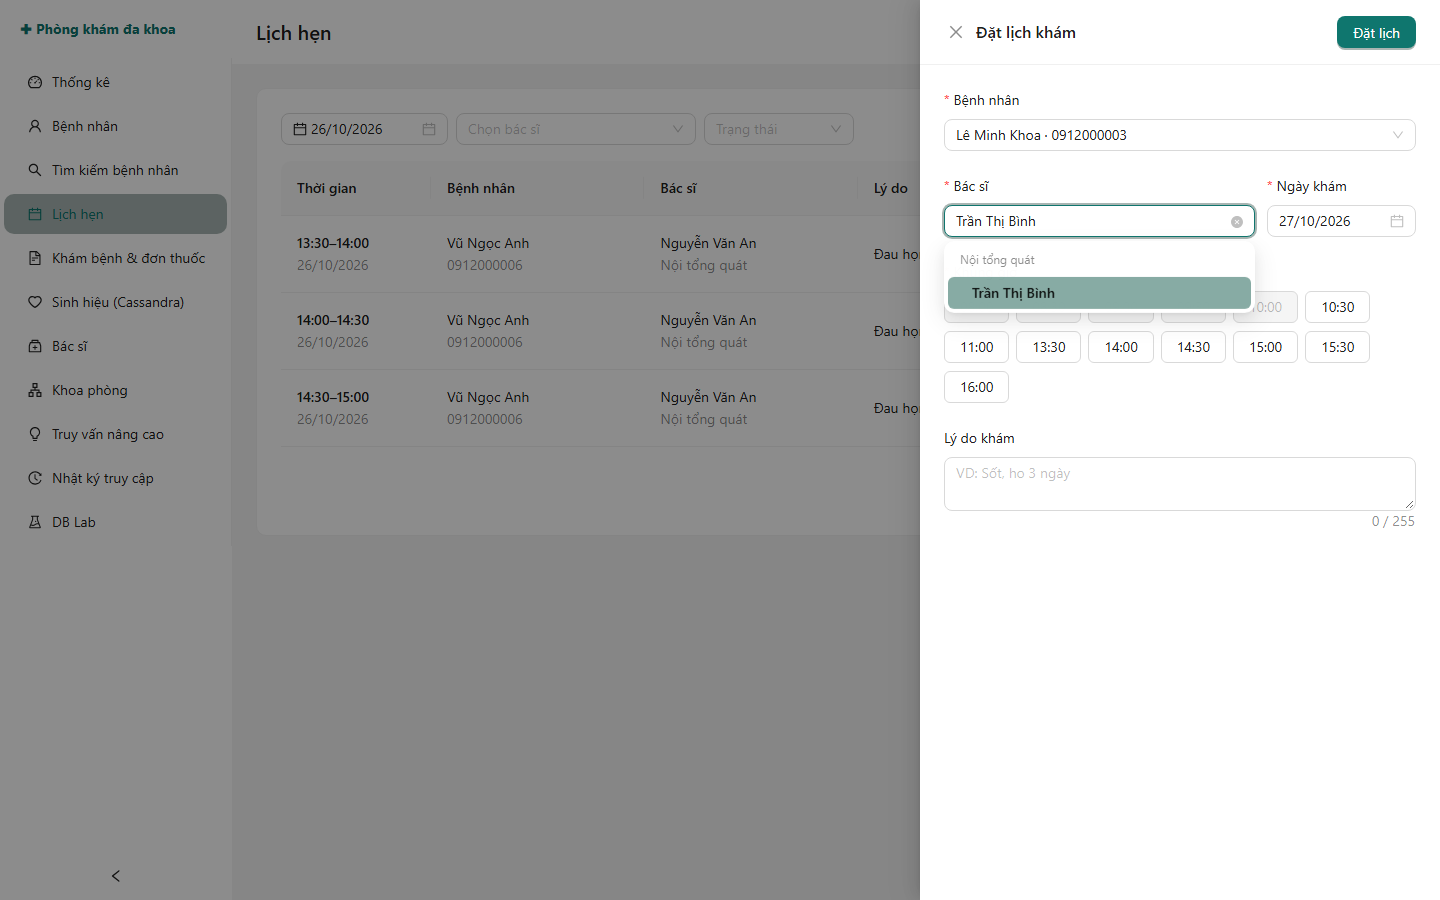
\includegraphics[width=0.95\linewidth]{4-4-fr3-booking.png}
\caption{FR3: đặt lịch với lưới khung giờ trống}
\label{fig:fr3-booking}
\end{figure}

\begin{figure}[H]
\centering
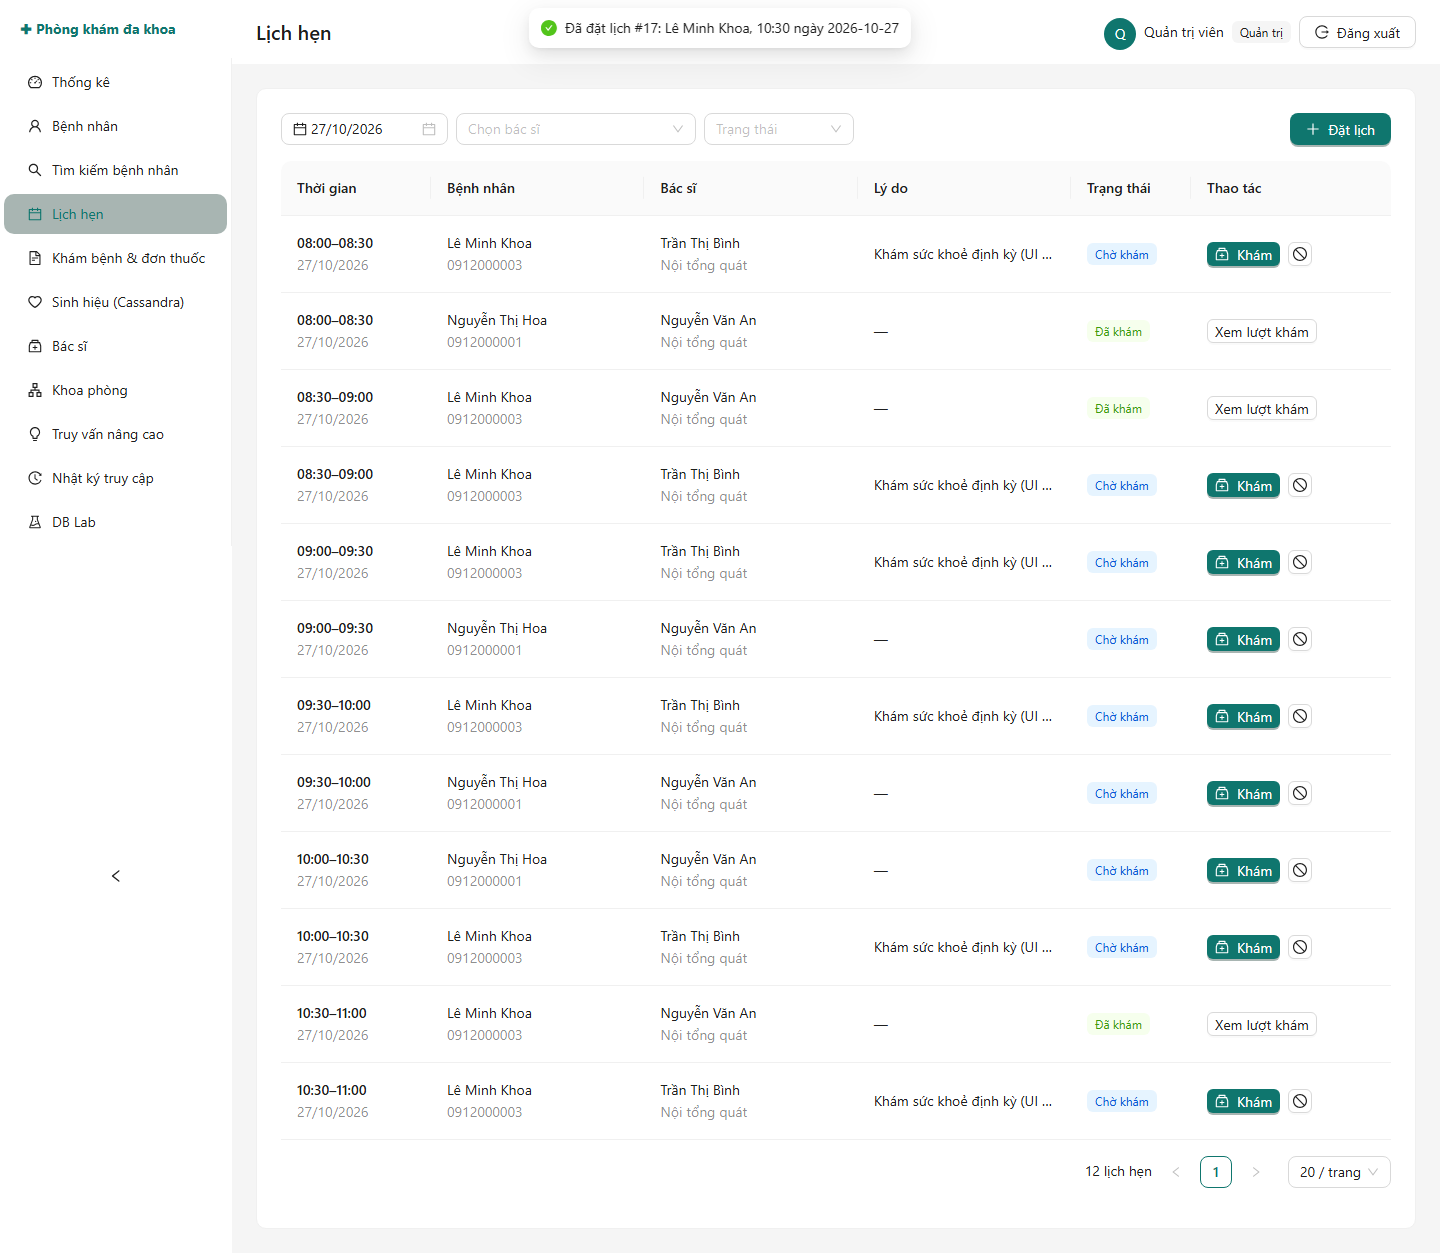
\includegraphics[width=0.95\linewidth]{4-4-fr3-appointments.png}
\caption{FR3: danh sách lịch hẹn}
\label{fig:fr3-list}
\end{figure}

\subsubsection{FR4 và FR6: Khám bệnh và chi tiết lượt khám}
Từ lịch hẹn, bác sĩ bấm \textit{Khám}, form có sẵn bệnh nhân và lý do khám. Bác sĩ nhập chẩn đoán và kê đơn (mỗi thuốc hiện tồn kho), form xem trước hoá đơn (Hình~\ref{fig:fr4}). \texttt{POST /visits} ghi trong \textbf{một transaction}:
\begin{enumerate}
    \item Ghi lượt khám.
    \item Ghi đơn thuốc.
    \item Với mỗi thuốc: \texttt{UPDATE medicines SET stock\_quantity = stock\_quantity - @qty WHERE \ldots{} AND stock\_quantity >= @qty} (kiểm tra và trừ trong một câu, nên không bị lost update), rồi ghi dòng đơn thuốc với giá tại thời điểm kê.
    \item Ghi hoá đơn.
    \item Đóng lịch hẹn.
\end{enumerate}

\begin{lstlisting}[language=SQL, caption={Kiểm tra và trừ tồn kho trong một câu lệnh (\texttt{visits.repository.js})}, label={lst:dispense}]
UPDATE dbo.medicines SET stock_quantity = stock_quantity - @qty
OUTPUT INSERTED.name, INSERTED.unit_price AS unitPrice
WHERE medicine_id = @id AND stock_quantity >= @qty;
\end{lstlisting}

Nếu câu lệnh không cập nhật dòng nào thì thuốc không đủ tồn kho; service ném lỗi 409 và \texttt{withTransaction()} rollback toàn bộ các bước đã ghi trước đó.
Thiếu thuốc ở bất kỳ bước nào thì \textbf{không ghi gì cả}, kèm thông báo nêu tên thuốc. Chi tiết lượt khám lấy bằng \textbf{một câu join 10 bảng} (Hình~\ref{fig:fr6}). Thu ngân bấm \textit{Thanh toán} trên hoá đơn.

\begin{figure}[H]
\centering
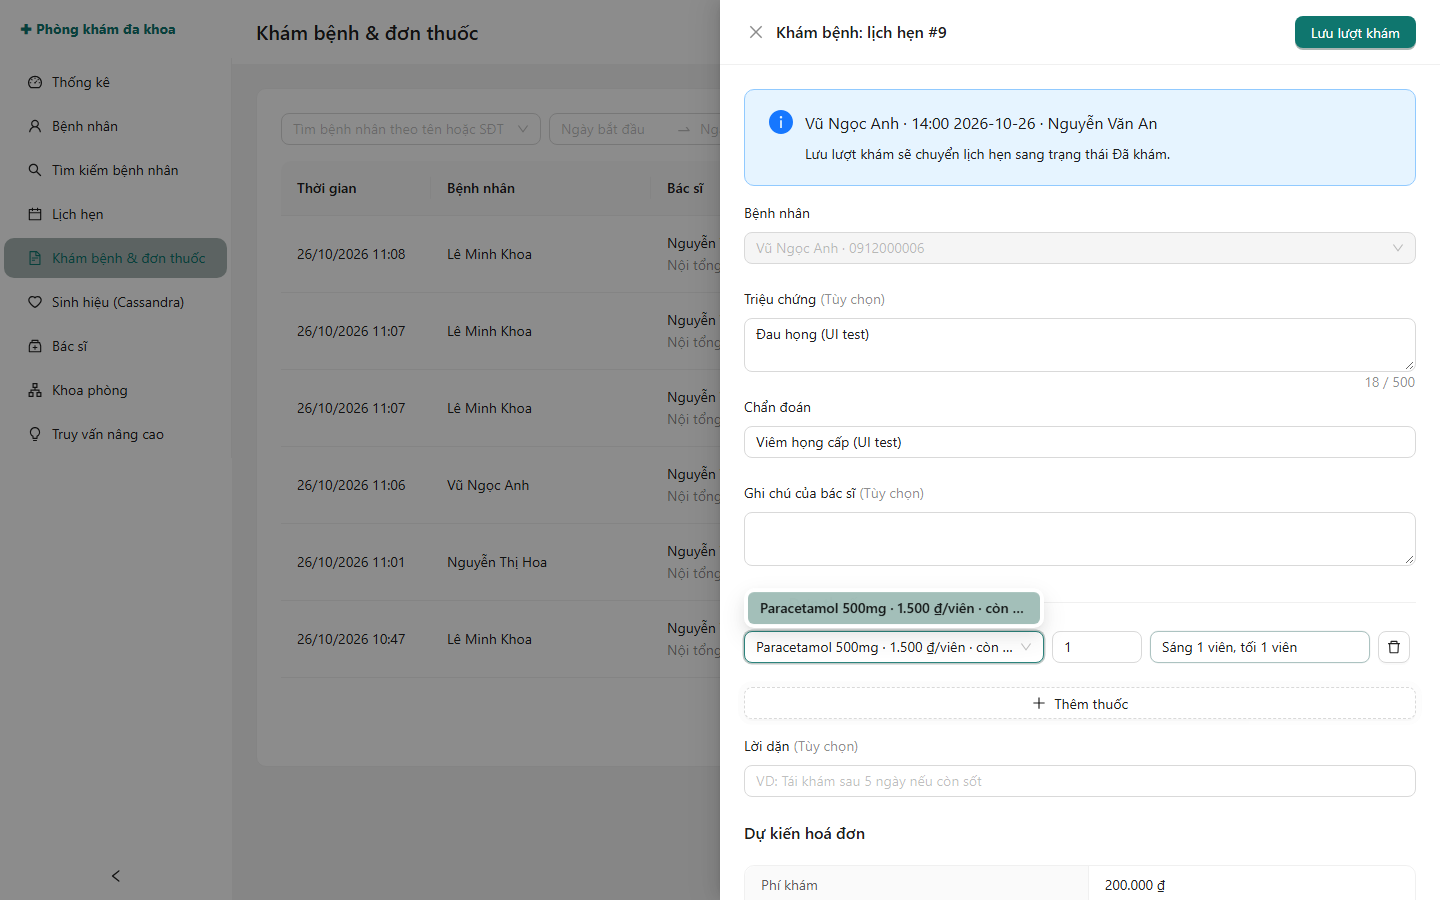
\includegraphics[width=0.95\linewidth]{4-4-fr4-visit-form.png}
\caption{FR4: form khám bệnh và kê đơn}
\label{fig:fr4}
\end{figure}

\begin{figure}[H]
\centering
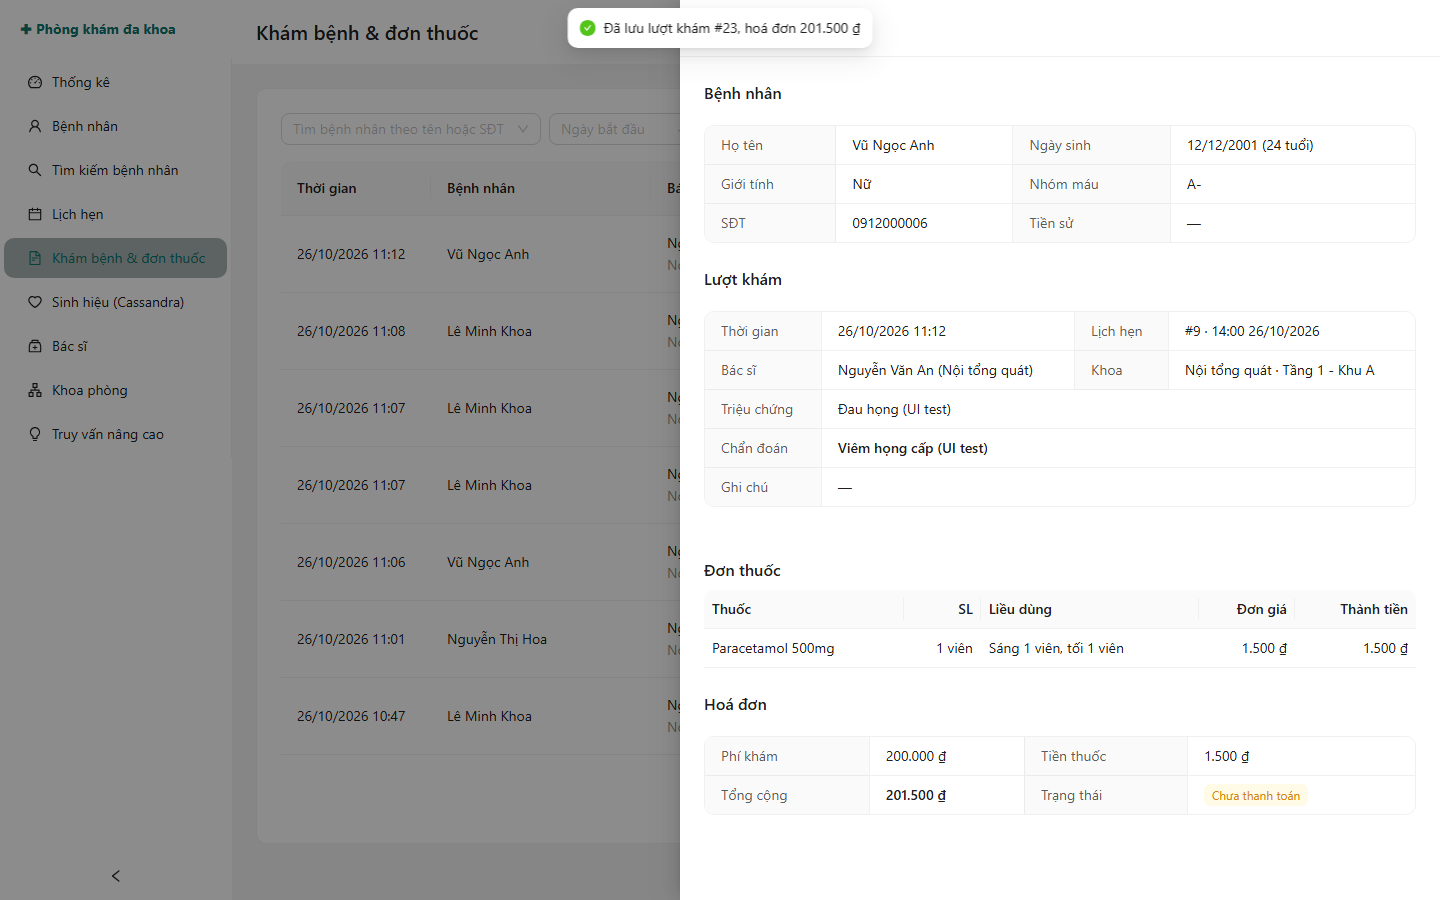
\includegraphics[width=0.95\linewidth]{4-4-fr6-visit-detail.png}
\caption{FR6: chi tiết lượt khám}
\label{fig:fr6}
\end{figure}

\subsubsection{FR9: Theo dõi sinh hiệu}
Thiết bị (trình giả lập trong app) gửi chỉ số. Mỗi lần đo được ghi bằng \textbf{logged batch} vào 3 bảng Cassandra: lịch sử theo (bệnh nhân, ngày), giá trị mới nhất (\texttt{USING TIMESTAMP} = thời điểm đo), cảnh báo theo ngày nếu vượt ngưỡng. Trang theo dõi nhận dữ liệu \textbf{trực tiếp qua Server-Sent Events}, vẽ biểu đồ nhịp tim/SpO$_2$/huyết áp, tô đỏ chỉ số bất thường và liệt kê cảnh báo trong ngày (Hình~\ref{fig:fr9}).

\begin{figure}[H]
\centering
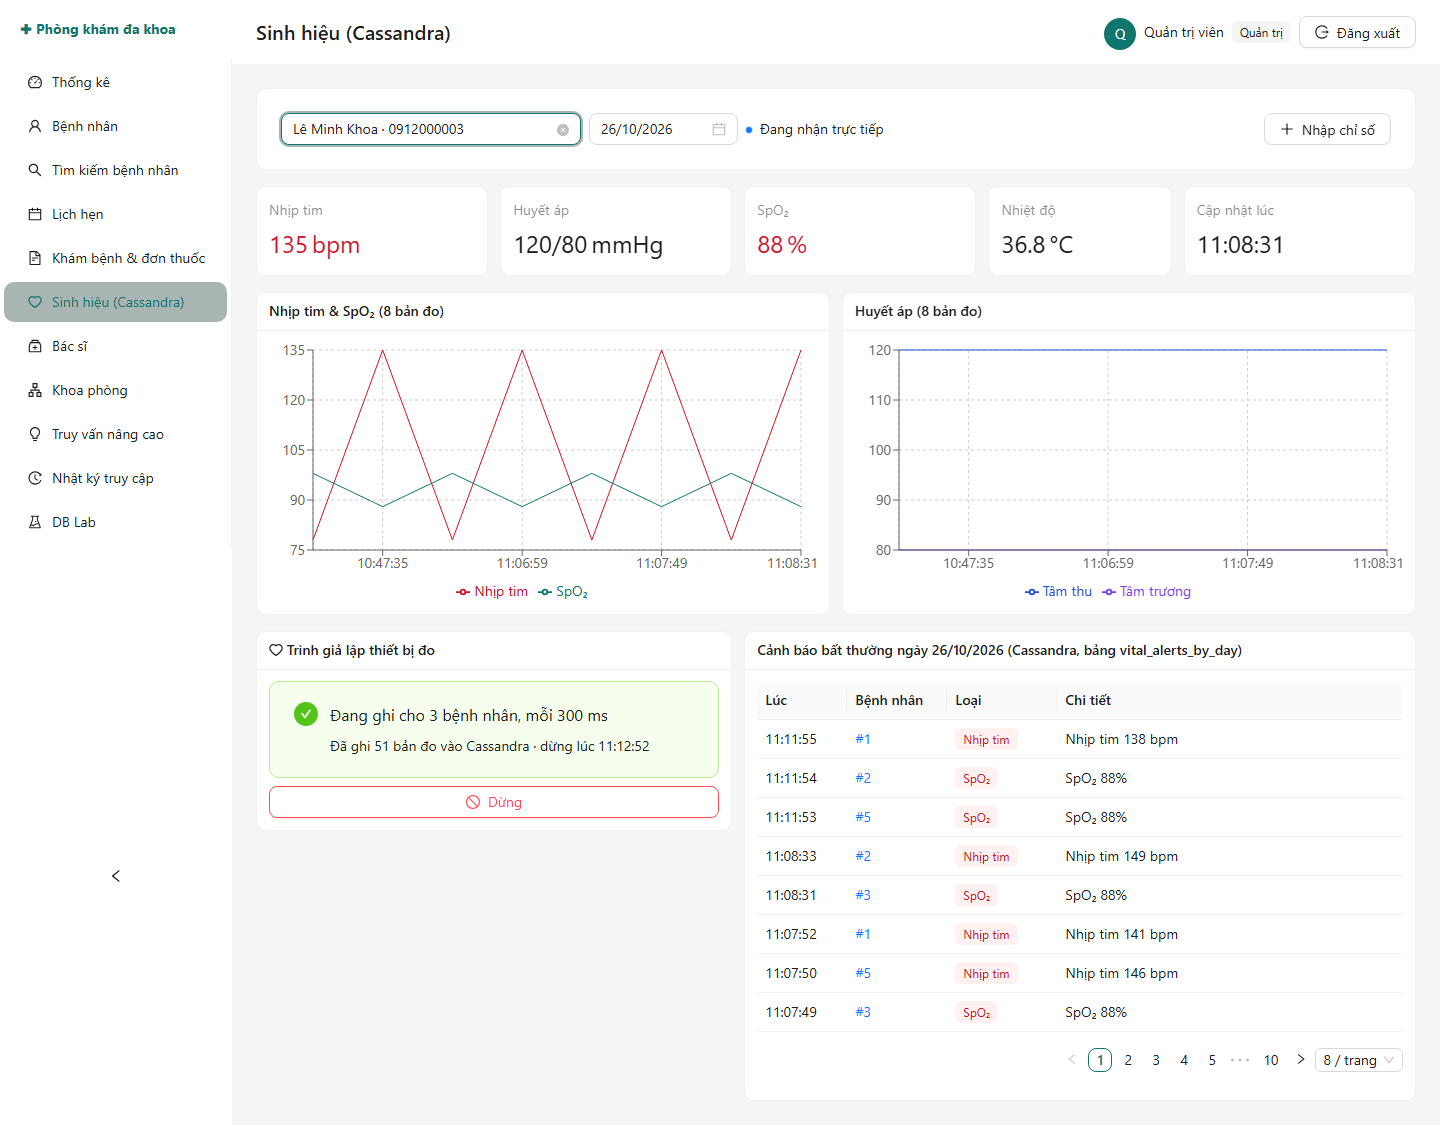
\includegraphics[width=0.95\linewidth]{4-4-fr9-vitals.png}
\caption{FR9: theo dõi sinh hiệu real-time}
\label{fig:fr9}
\end{figure}

\subsubsection{Nhật ký truy cập}
Middleware ghi mỗi request API (bất đồng bộ, không làm chậm request) vào bảng \texttt{access\_logs\_by\_user\_day} (partition theo người dùng + ngày, TTL 90 ngày). Quản trị xem nhật ký theo người dùng và ngày (Hình~\ref{fig:logs}).

\begin{figure}[H]
\centering
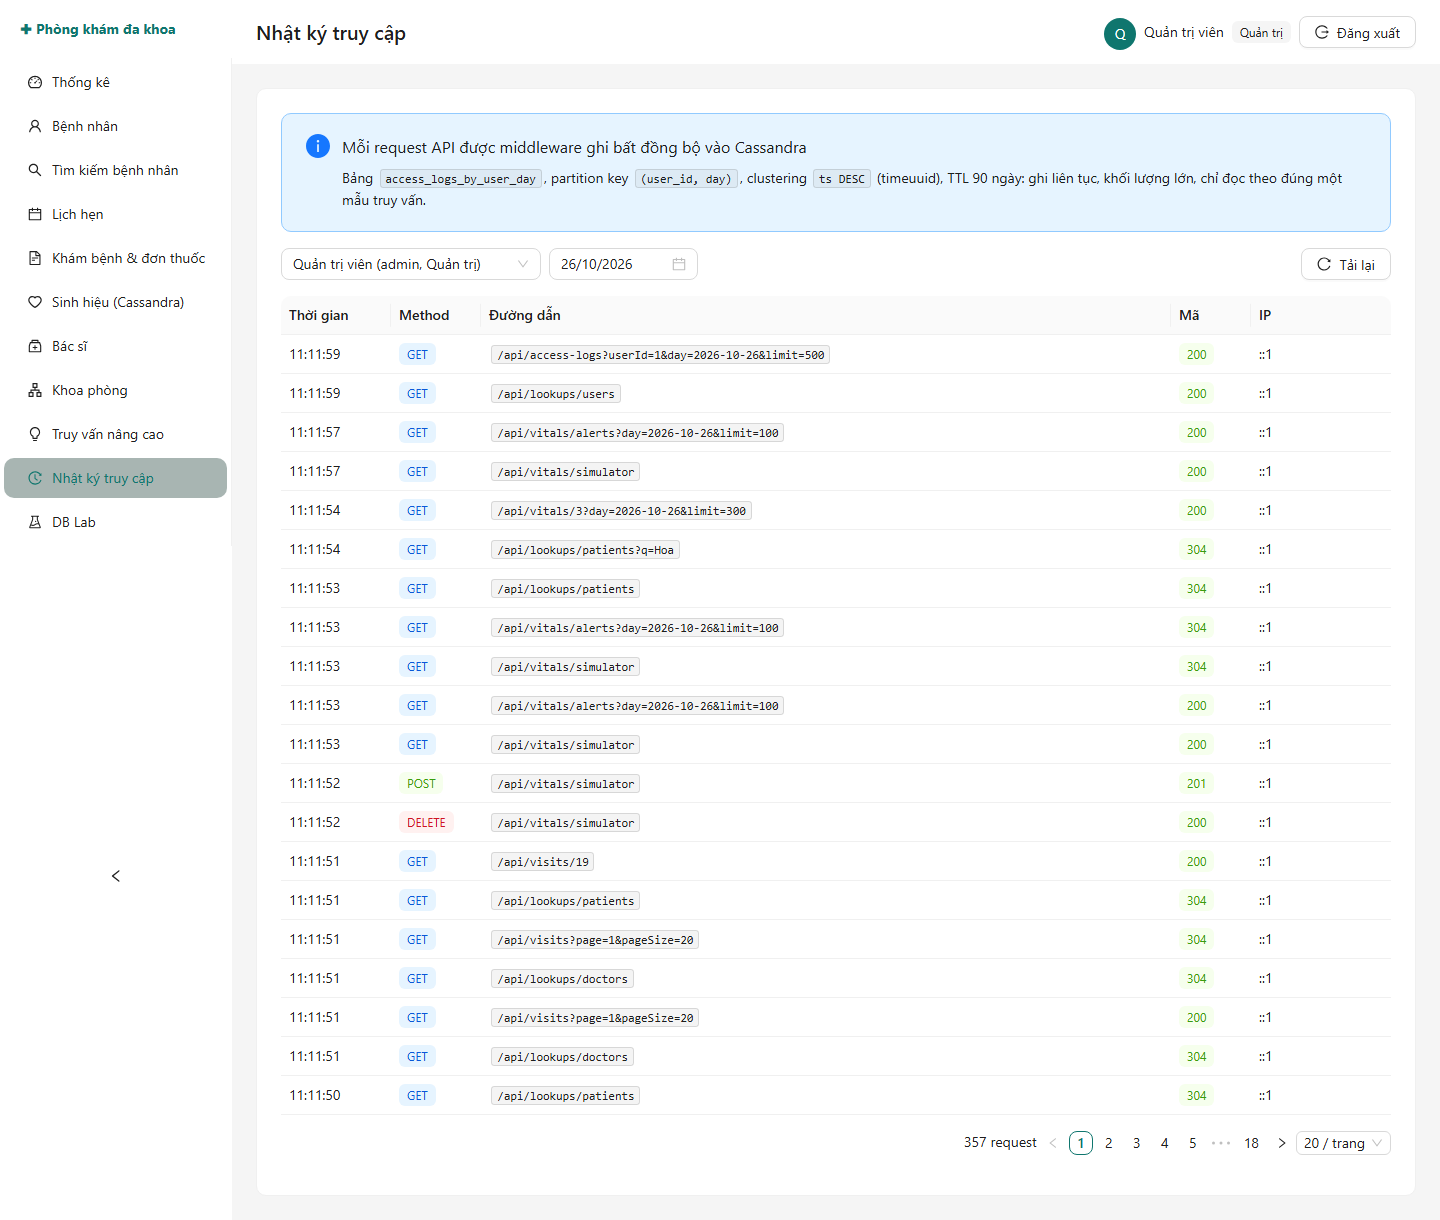
\includegraphics[width=0.95\linewidth]{4-4-access-logs.png}
\caption{Nhật ký truy cập (Cassandra)}
\label{fig:logs}
\end{figure}

\subsubsection{FR1, FR2, FR5, FR7, FR8}
\todo{Dương}{Mô tả hiện thực và ảnh giao diện cho FR1 Bệnh nhân, FR2 Bác sĩ, FR5 Tìm kiếm, FR7 Thống kê, FR8 Truy vấn nâng cao.}

\subsection{Ma trận 8 loại truy vấn}
\label{sec:query-matrix}
\todo{Dương}{Bảng 8 loại a--h (Insert, Delete, Update, Query 1 điều kiện, Query đa điều kiện, Join, Subquery, Aggregate): mỗi loại $\rightarrow$ endpoint, câu SQL/CQL tiêu biểu, chức năng và màn hình tương ứng. Gợi ý nguồn: mục 2 của \texttt{docs/testing/checklist.md}.}

\subsection{DB Lab: đưa nghiên cứu vào ứng dụng}
Trang DB Lab (chỉ ADMIN) chạy các thí nghiệm của Mục~\ref{sec:demo} \textbf{bằng chính code dùng cho script demo} (\texttt{server/src/modules/lab/}), trên một connection pool riêng để thiết lập phiên (isolation, lock timeout) không ảnh hưởng ứng dụng. Mỗi thời điểm chỉ chạy một thí nghiệm.

\begin{table}[H]
\centering
\caption{Các tab của DB Lab}
\label{tab:dblab}
\begin{tabularx}{\linewidth}{|p{3.4cm}|X|}
\hline
\textbf{Tab} & \textbf{Thí nghiệm} \\ \hline
iv. Transaction & Quy trình khám 5 bước, chọn bước gây lỗi; so sánh SQL Server (ROLLBACK, dữ liệu trước = sau) với Cassandra (dở dang / batch) \\ \hline
v. Concurrency & Ma trận hiện tượng $\times$ mức cô lập; đặt trùng lịch $N$ request theo 5 cách; tạo deadlock và xem khoá \\ \hline
vi. Backup \& recovery & Backup full/diff/log, lịch sử msdb; point-in-time restore sau sự cố ``UPDATE quên WHERE'' \\ \hline
i--iii & \colorbox{yellow!40}{TODO (Dương): lưu trữ, chỉ mục, kế hoạch thực thi} \\ \hline
\end{tabularx}
\end{table}

\begin{figure}[H]
\centering
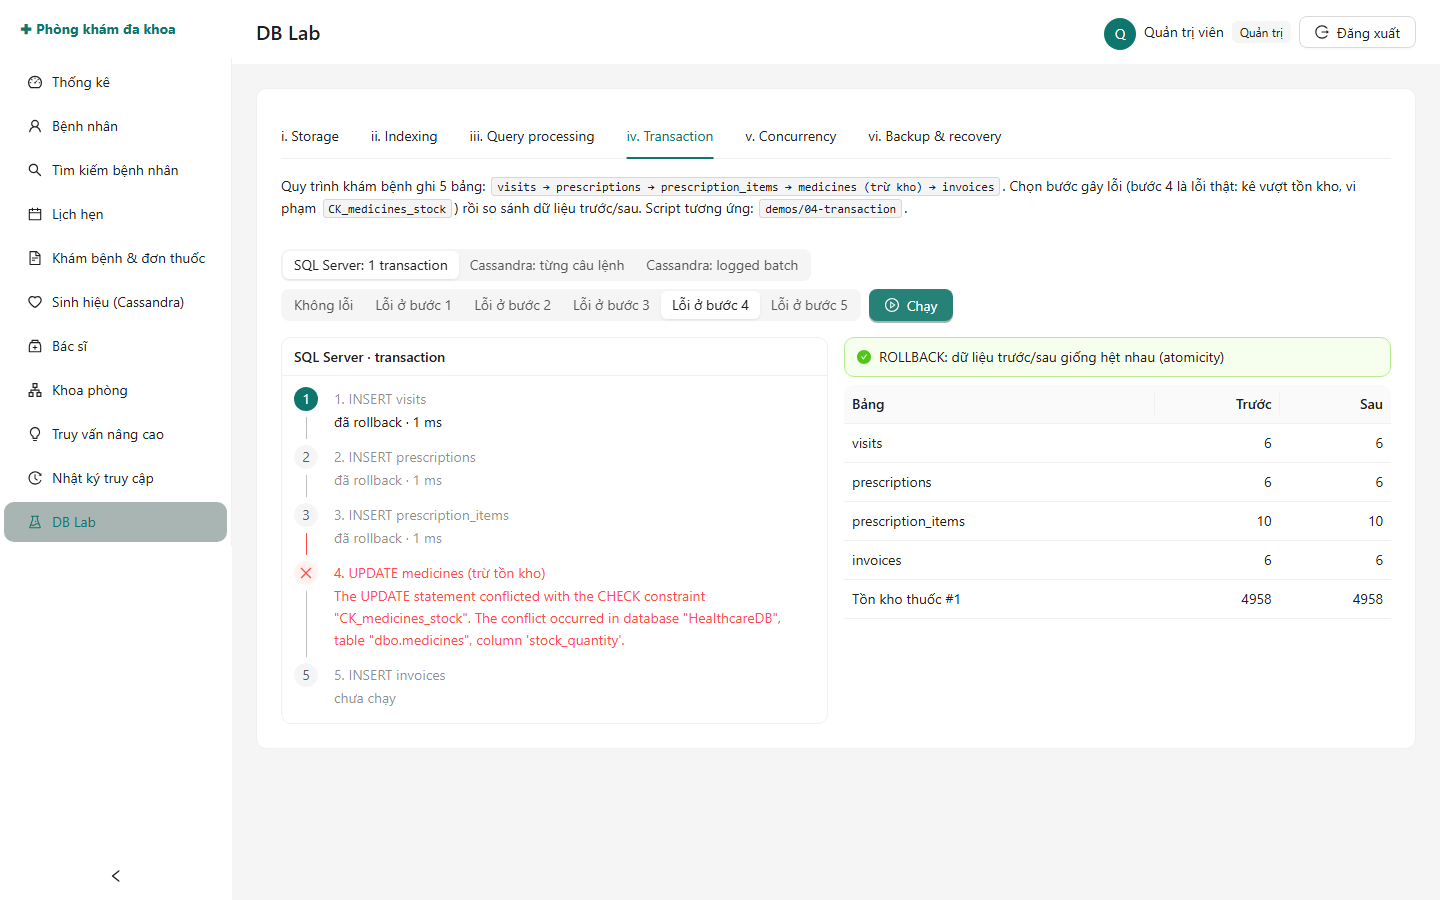
\includegraphics[width=0.95\linewidth]{4-6-lab-transaction.png}
\caption{DB Lab: tab Transaction}
\label{fig:lab-tx}
\end{figure}

\begin{figure}[H]
\centering
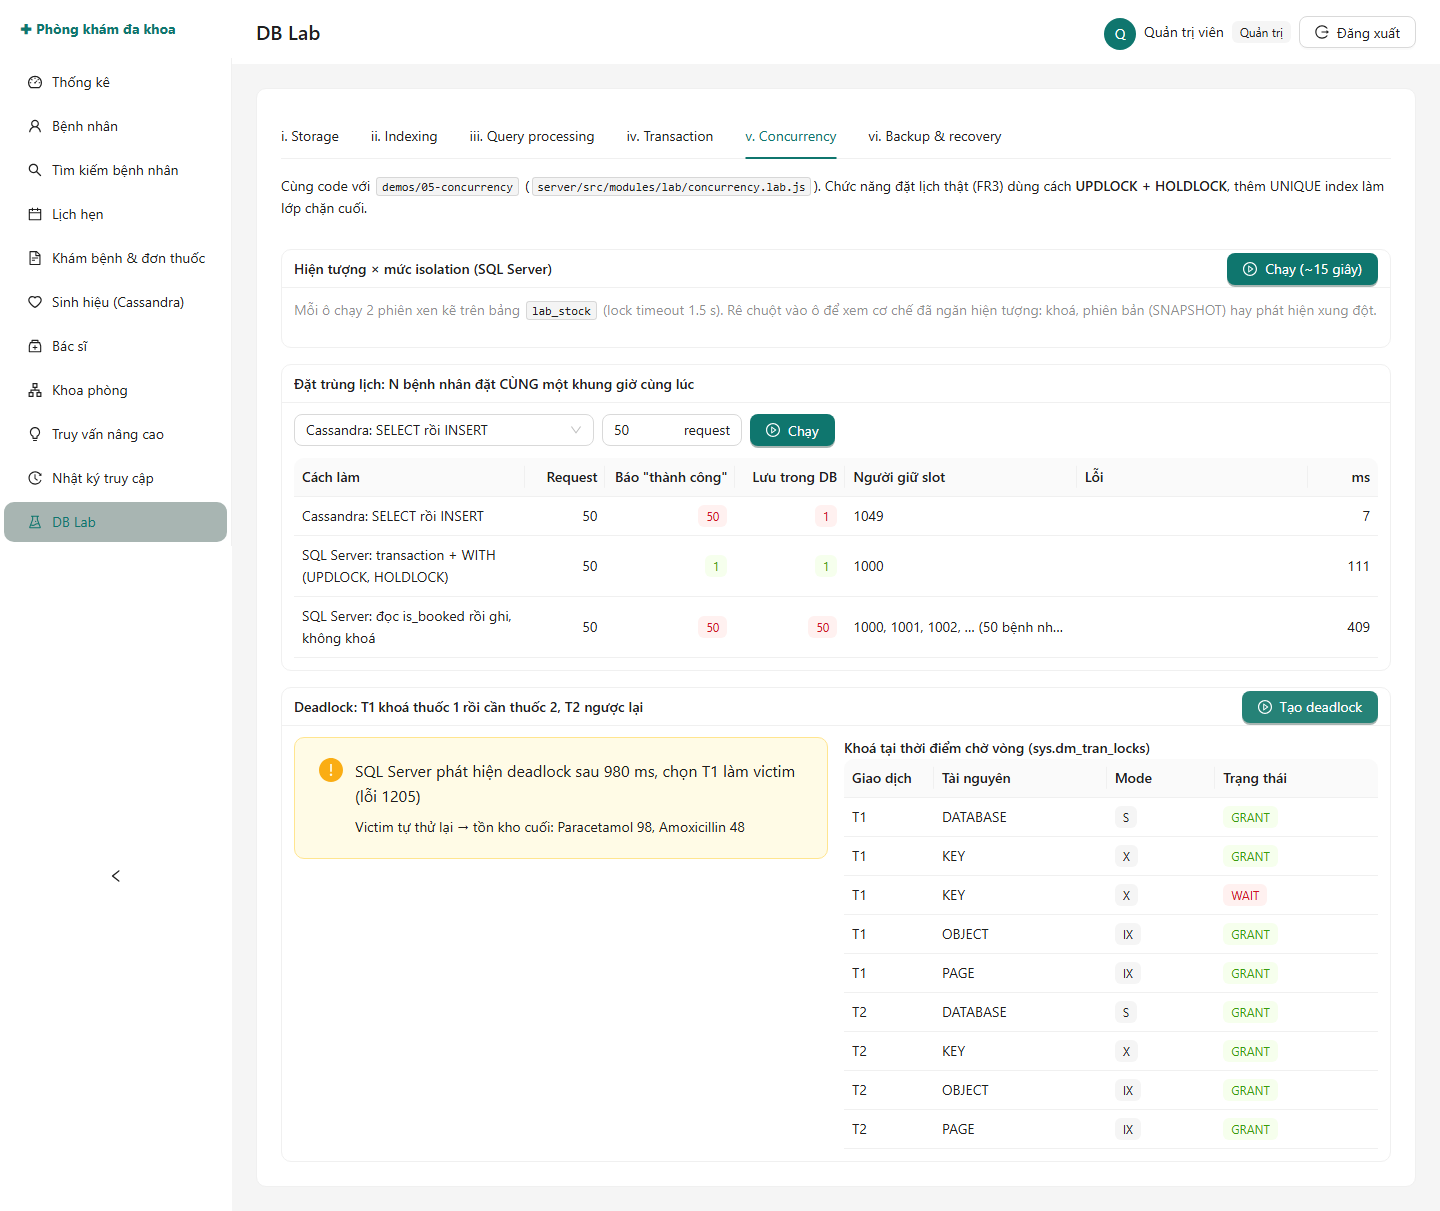
\includegraphics[width=0.95\linewidth]{4-6-lab-concurrency.png}
\caption{DB Lab: tab Concurrency}
\label{fig:lab-cc}
\end{figure}

\begin{figure}[H]
\centering
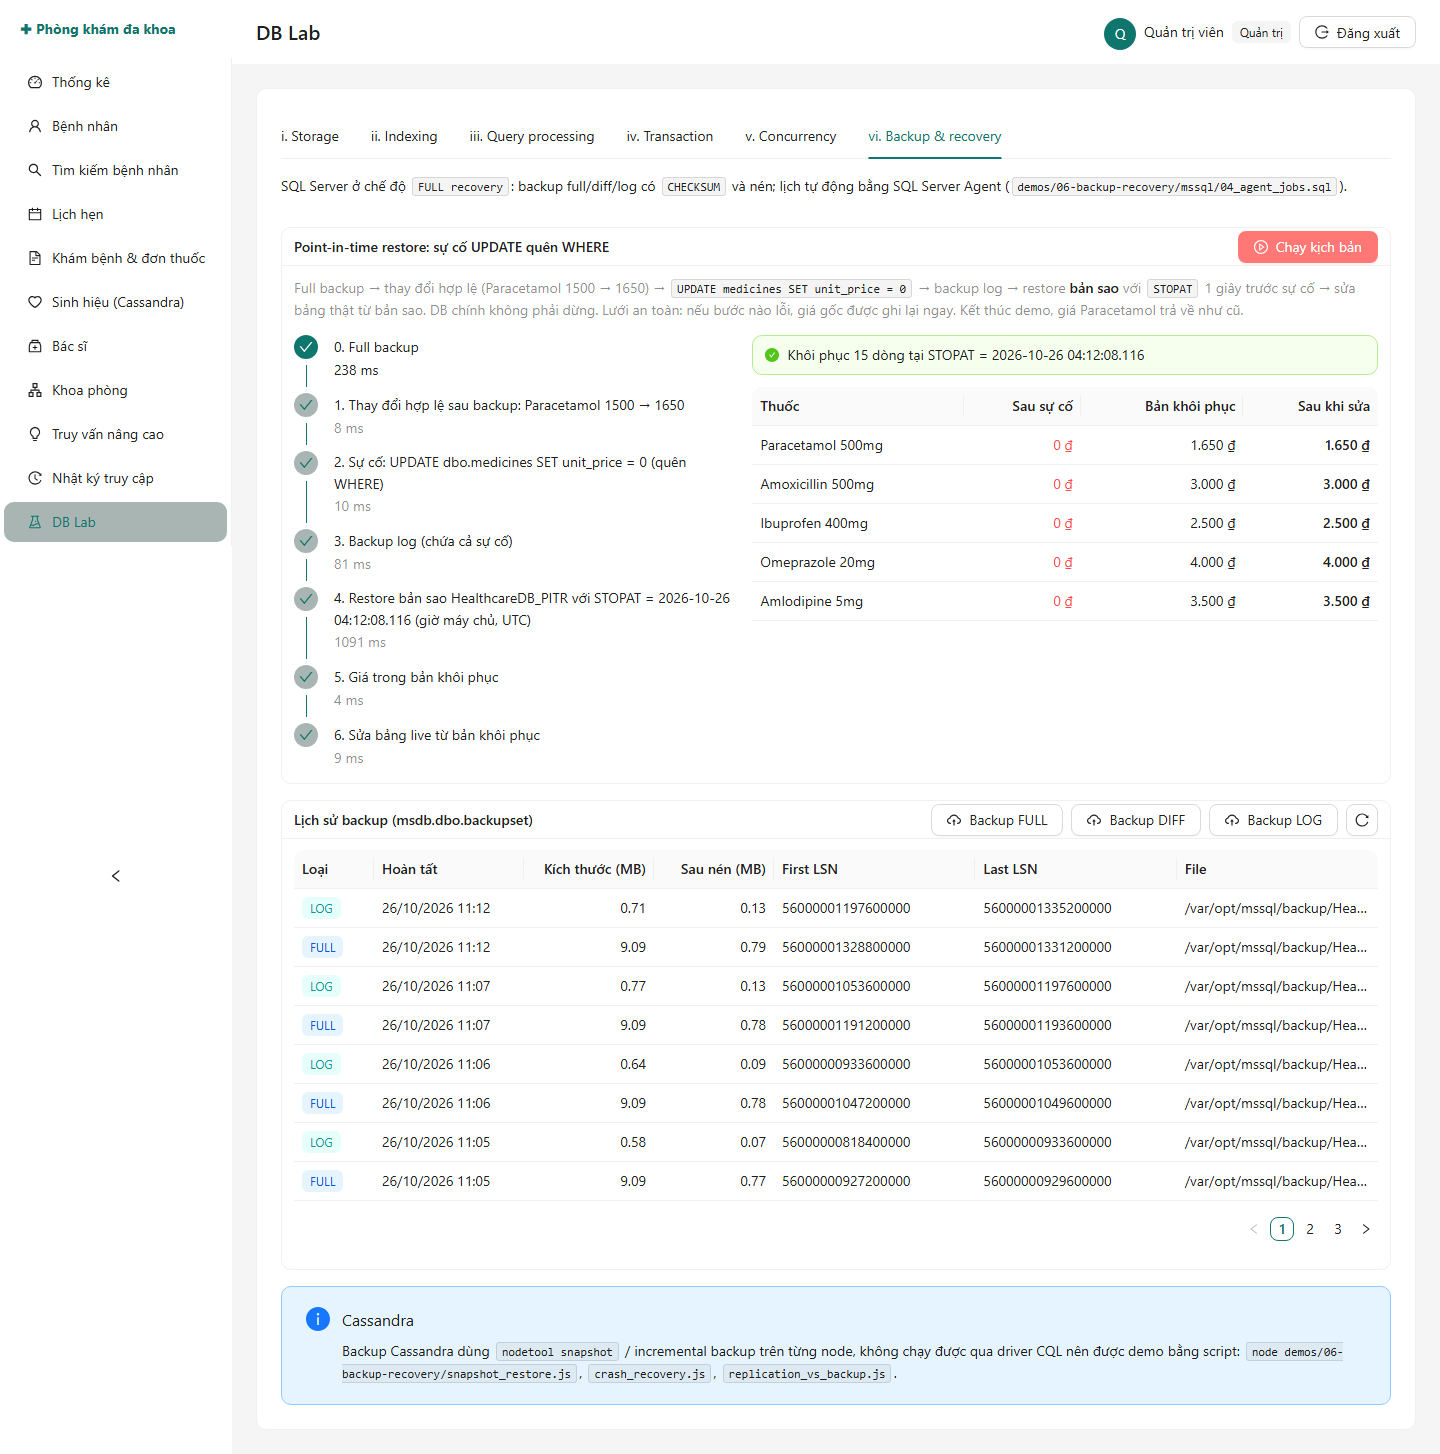
\includegraphics[width=0.95\linewidth]{4-6-lab-backup.png}
\caption{DB Lab: tab Backup \& recovery}
\label{fig:lab-backup}
\end{figure}

\subsection{Kiểm thử}
Ứng dụng được kiểm thử ở hai mức:
\begin{itemize}
    \item \textbf{Test API end-to-end} (\texttt{server/test/hoang-features.e2e.test.js}, chạy bằng \texttt{npm run test:e2e -w server}): 14 test gọi API thật trên hai DB đang chạy. Kết quả: \textbf{14/14 đạt}.
    \item \textbf{Kiểm thử giao diện} bằng trình duyệt headless (Playwright) trên 9 luồng nghiệp vụ: \textbf{0 lỗi console}.
    \item \textbf{Test chéo thủ công} theo checklist 24 ca (\texttt{docs/testing/checklist.md}): mỗi thành viên kiểm thử chức năng của người kia.
\end{itemize}

\begin{table}[H]
\centering
\caption{Các ca kiểm thử API tiêu biểu}
\label{tab:e2e}
\begin{tabularx}{\linewidth}{|p{3cm}|X|X|}
\hline
\textbf{Chức năng} & \textbf{Ca kiểm thử} & \textbf{Kết quả mong đợi} \\ \hline
FR3 Đặt lịch & 20 request đặt \textbf{cùng một} khung giờ gửi đồng thời & Đúng 1 thành công (201), 19 nhận 409 \\ \hline
FR3 Đặt lịch & Đặt lại khung giờ đã có lịch; xoá lịch đang chờ; huỷ rồi xoá & 409; 409; khung giờ mở lại, xoá được (204) \\ \hline
FR3 Đặt lịch & Đặt khung giờ đã qua; dữ liệu sai kiểu & 400 kèm chi tiết lỗi \\ \hline
FR4 Khám bệnh & Kê đơn hợp lệ 2 thuốc từ lịch hẹn & Hoá đơn = phí khám + tiền thuốc; tồn kho giảm đúng; lịch hẹn \textit{Đã khám} \\ \hline
FR4 Khám bệnh & Kê Salbutamol vượt tồn kho & 409 nêu tên thuốc; tồn kho và số lượt khám \textbf{không đổi} \\ \hline
FR6 Chi tiết & Lấy chi tiết lượt khám vừa tạo, thanh toán 2 lần & Đủ bệnh nhân, khoa, hoá đơn; lần thanh toán thứ 2 nhận 409 \\ \hline
FR9 Sinh hiệu & Ghi nhịp tim 135, SpO$_2$ 88; mở luồng SSE & Sinh 2 cảnh báo; luồng SSE đẩy bản đo mới \\ \hline
Nhật ký & Gọi API bằng một tài khoản & Mọi request được ghi, token bị che \\ \hline
Phân quyền & Bác sĩ đặt lịch; bác sĩ gọi API DB Lab & 403 \\ \hline
\end{tabularx}
\end{table}

Các lỗi phát hiện trong quá trình kiểm thử và đã sửa: luồng SSE bị proxy của Vite giữ header nên trang sinh hiệu không nhận dữ liệu; phí khám dự kiến hiển thị bằng 0 với tài khoản bác sĩ; Vite 8 bị crash native khi hot reload nên hạ về Vite 7.

\section{Làm việc nhóm}
\label{sec:teamwork}

\subsection{Phân công và đóng góp}

\begin{table}[H]
\centering
\caption{Phân công và tỉ lệ đóng góp}
\label{tab:contrib}
\begin{tabularx}{\linewidth}{|p{3.2cm}|X|X|}
\hline
\textbf{Hạng mục} & \textbf{Hoàng} & \textbf{Dương} \\ \hline
Chủ đề DBMS & iv, v, vi & i, ii, iii \\ \hline
Chức năng ứng dụng & FR3, FR4, FR6, FR9, nhật ký truy cập & FR1, FR2, FR5, FR7, FR8 \\ \hline
DB Lab & Tab iv--vi & Tab i--iii \\ \hline
Hạ tầng \& quy trình & Docker, skeleton, auth, quy trình Git, bộ đo hiệu năng, kiểm thử & Mô hình Cassandra, bộ sinh dữ liệu lớn \\ \hline
Báo cáo & Mục 1, 2.1, 3.4--3.6, 4.1, 4.2, 4.4, 4.6, 4.7, 5, Phụ lục & Mục 2.2, 3.1--3.3, 4.3, 4.4, 4.5 \\ \hline
\textbf{Tỉ lệ đóng góp tự đánh giá} & \colorbox{yellow!40}{TODO: \_\_\%} & \colorbox{yellow!40}{TODO: \_\_\%} \\ \hline
\end{tabularx}
\end{table}

\subsection{Quy trình làm việc}
\begin{itemize}
    \item \textbf{Kế hoạch:} \texttt{docs/PLAN.md} là nguồn sự thật duy nhất về phạm vi, phân công và tiến độ. Mỗi bước có ID (ví dụ \texttt{S3.3}, \texttt{T4.3}), người phụ trách, input, output, điều kiện hoàn thành, hạn và trạng thái.
    \item \textbf{Nhật ký công việc:} \texttt{docs/TRACKLOG.md}, mỗi người một bảng riêng, chỉ ghi thêm. Mỗi dòng trỏ tới output kiểm chứng được (file, PR, kết quả đo).
    \item \textbf{GitHub Flow:} mỗi bước là một branch và một Pull Request, người kia review trong 24 giờ rồi squash merge; nhánh \texttt{main} được bảo vệ, không ai push thẳng. Commit và branch đều mang ID bước để truy vết. CODEOWNERS phân vùng thư mục theo người sở hữu để hai người làm song song không xung đột.
    \item \textbf{Họp:} thứ 2 và thứ 5 hằng tuần lúc 21:00, có biên bản sau mỗi buổi (Phụ lục~\ref{app:meetings}).
\end{itemize}

\subsection{Nhật ký công việc}
Bảng~\ref{tab:tracklog-hoang} tóm tắt nhật ký của Hoàng, trích từ \texttt{docs/TRACKLOG.md}; mỗi dòng tương ứng một commit trên GitHub.

\begin{table}[H]
\centering
\caption{Nhật ký công việc của Hoàng}
\label{tab:tracklog-hoang}
\small
\begin{tabularx}{\linewidth}{|p{1.6cm}|p{2.2cm}|X|c|}
\hline
\textbf{Ngày} & \textbf{Bước} & \textbf{Việc đã làm và output} & \textbf{Giờ} \\ \hline
26/10/2026 & S0.1--S0.4 & Khởi tạo repo, Docker Compose 2 DBMS (+ cluster 3 node), quy trình Git, skeleton Express + React, đăng nhập JWT, module mẫu Khoa phòng, ghi nhật ký vào Cassandra & 3.75 \\ \hline
26/10/2026 & S1.1, S1.2, S1.5 & Bản nháp 9 FR và ma trận 8 loại truy vấn, ERD và schema SQL Server, API contract & 2 \\ \hline
26/10/2026 & S1.6 & Bộ đo hiệu năng dùng chung: latency, logical reads, throughput song song, xuất CSV & 1 \\ \hline
26/10/2026 & T4.1--T4.5 & Chủ đề Transaction: 9 kịch bản trên 2 DBMS, đo torn read và chi phí transaction & 3 \\ \hline
26/10/2026 & T5.1--T5.5 & Chủ đề Concurrency: ma trận 5 hiện tượng $\times$ 5 mức cô lập, double-booking, leo thang khoá, deadlock, last-write-wins, tunable consistency & 3 \\ \hline
26/10/2026 & T6.1--T6.5 & Chủ đề Backup \& recovery: recovery model, chuỗi sao lưu, point-in-time restore, crash recovery, snapshot, replication $\neq$ backup, Agent job & 3 \\ \hline
26/10/2026 & S3.3, S3.4, S3.6, S3.9, S3.11, S3.12 & Backend và giao diện FR3, FR4, FR6, FR9, nhật ký truy cập, DB Lab iv--vi; 14 test E2E, kiểm thử giao diện headless & 8 \\ \hline
26/10/2026 & S4.1, S5.1--S5.4 & Checklist test chéo 24 ca, bản nháp báo cáo, 9 ảnh giao diện, chuẩn bị họp kickoff & 2 \\ \hline
\end{tabularx}
\end{table}

\todo{Dương}{Bảng nhật ký công việc của Dương (cùng định dạng Bảng~\ref{tab:tracklog-hoang}).}

\subsection{Các buổi họp}

\begin{table}[H]
\centering
\caption{Danh sách các buổi họp}
\label{tab:meetings}
\begin{tabularx}{\linewidth}{|c|p{2.2cm}|X|}
\hline
\textbf{\#} & \textbf{Ngày} & \textbf{Nội dung chính} \\ \hline
1 & 26/10/2026 & Kickoff: chốt DBMS, chủ đề, phân công, timeline, quy trình; Hoàng báo cáo phần đã làm; Dương chạy repo trên máy mình \\ \hline
\multicolumn{3}{|l|}{\colorbox{yellow!40}{TODO: bổ sung các buổi họp tiếp theo}} \\ \hline
\end{tabularx}
\end{table}

\subsection{Khó khăn và cách xử lý}

\begin{table}[H]
\centering
\caption{Khó khăn và cách xử lý}
\begin{tabularx}{\linewidth}{|X|X|}
\hline
\textbf{Khó khăn} & \textbf{Cách xử lý} \\ \hline
2 người làm khối lượng của nhóm 4--5 người & Ưu tiên theo MoSCoW, phân vùng sở hữu thư mục để làm song song không xung đột \\ \hline
Script demo gây hỏng dữ liệu khi một bước lỗi (backup) & Dừng ở lỗi đầu tiên, kiểm tra điều kiện trước các bước có thể làm mất dữ liệu, tự khôi phục dữ liệu trong ứng dụng (Mục~\ref{sec:backup}) \\ \hline
Gỡ cluster Cassandra sai cách làm mất dữ liệu dev & Script gỡ dùng \texttt{decommission -{}-force}, dừng nếu lỗi, đã kiểm chứng giữ đủ dữ liệu \\ \hline
\texttt{db:init} lỗi timeout vì Cassandra khởi động chậm & \texttt{db:up} chờ container \textit{healthy} (\texttt{-{}-wait}); \texttt{db:init} tự thử kết nối lại tới 3 phút \\ \hline
\end{tabularx}
\end{table}

\section{Kết luận và tự đánh giá}
\label{sec:conclusion}

\subsection{Kết luận}
Kết quả thực nghiệm trên sáu chủ đề cho thấy hai hệ quản trị có thế mạnh ở các nhóm dữ liệu khác nhau của phòng khám, do đó hệ thống sử dụng đồng thời cả hai với vai trò như sau:

\begin{itemize}
    \item \textbf{Dữ liệu lâm sàng và tài chính} (lịch hẹn, lượt khám, đơn thuốc, tồn kho, hoá đơn) nên đặt trên \textbf{SQL Server}. Các nghiệp vụ này bắt buộc atomic trên nhiều bảng (Mục~\ref{sec:transaction}), có tài nguyên khan hiếm bị nhiều người tranh như khung giờ khám và tồn kho (Mục~\ref{sec:concurrency}), và cần khôi phục tới từng giây khi người dùng thao tác nhầm (Mục~\ref{sec:backup}). Cassandra không có transaction nhiều partition, không có rollback, và nếu không dùng LWT thì các yêu cầu ghi đồng thời ghi đè lên nhau mà không báo lỗi.
    \item \textbf{Dữ liệu thiết bị và hệ thống} (sinh hiệu, nhật ký truy cập) phù hợp với \textbf{Cassandra}. Dữ liệu chỉ ghi thêm, mỗi bệnh nhân có một nguồn ghi nên last-write-wins chấp nhận được, chỉ cần atomic trong một lần đo (logged batch), và cần \textit{luôn ghi được} kể cả khi mất một node nhờ replication. Throughput ghi của Cassandra cao hơn SQL Server nhiều lần ở cùng điều kiện (Bảng~\ref{tab:tx-cost}).
    \item Khi dữ liệu quan trọng buộc phải nằm trên Cassandra, phải dùng consistency QUORUM cho cả đọc lẫn ghi: thí nghiệm ở Bảng~\ref{tab:consistency} cho thấy đọc ở mức ONE bỏ sót thông tin dị ứng 3/5 lần.
\end{itemize}

Ứng dụng của nhóm hiện thực cách phân chia này theo mô hình \textit{polyglot persistence}: 8 chức năng nghiệp vụ trên SQL Server, sinh hiệu và nhật ký trên Cassandra. Các kỹ thuật rút ra từ thí nghiệm được dùng trực tiếp trong chức năng thật (khoá \texttt{UPDLOCK + HOLDLOCK} khi đặt lịch, trừ kho bằng một câu \texttt{UPDATE} có điều kiện, logged batch và \texttt{USING TIMESTAMP} cho sinh hiệu), và trang DB Lab cho phép chạy lại các thí nghiệm ngay trong ứng dụng.

\todo{Dương}{Bổ sung kết luận từ chủ đề i--iii (lưu trữ, chỉ mục, xử lý truy vấn) vào đoạn trên.}

\subsection{Tự đánh giá theo tiêu chí chấm điểm}

\begin{table}[H]
\centering
\caption{Tự đánh giá theo rubric}
\label{tab:self-assessment}
\begin{tabularx}{\linewidth}{|p{2.8cm}|c|X|c|}
\hline
\textbf{Tiêu chí} & \textbf{Trọng số} & \textbf{Minh chứng} & \textbf{Tự chấm} \\ \hline
Structure & 10\% & 6 mục (trong giới hạn 4--7), có Giới thiệu, Kết luận kèm tự đánh giá, Tài liệu tham khảo; phụ lục tách riêng & TODO \\ \hline
Content & 10\% & Ma trận truy vết ở Phụ lục~\ref{app:trace}: mọi yêu cầu của đề đều trỏ tới mục báo cáo và mã nguồn & TODO \\ \hline
Presentation & 10\% & Mỗi thành viên trình bày phần mình; demo trực tiếp trên DB Lab, có video dự phòng & TODO \\ \hline
Teamwork & 10\% & Bảng phân công và nhật ký công việc (Mục~\ref{sec:teamwork}), quy trình PR có review, biên bản họp ở Phụ lục~\ref{app:meetings} & TODO \\ \hline
Demonstration & 30\% & 6/6 chủ đề, mỗi chủ đề chạy trên cả hai DBMS, có số đo, bảng so sánh và kết luận; script chạy lại được & TODO \\ \hline
Application & 30\% & 9 chức năng (đề yêu cầu 4), đủ 8 loại truy vấn, kiến trúc n-tier phân lớp, validation, thông báo lỗi tiếng Việt, phân quyền, 14/14 test E2E đạt & TODO \\ \hline
Bonus & +2 & 4 chủ đề vượt yêu cầu; DB Lab đưa toàn bộ thí nghiệm vào ứng dụng & TODO \\ \hline
\end{tabularx}
\end{table}

\subsection{Hạn chế và hướng phát triển}
\textbf{Hạn chế:}
\begin{itemize}
    \item Mọi thí nghiệm chạy trên một máy, các node Cassandra là container trên cùng máy chủ. Độ trễ mạng giữa các node gần như bằng 0, nên số đo throughput và độ trễ của Cassandra lạc quan hơn một cụm thật.
    \item Các thí nghiệm đồng thời dùng số client nhỏ (tối đa 50); chưa đo hành vi khi tải kéo dài nhiều giờ.
    \item SQL Server chạy một instance, chưa thử nghiệm giải pháp sẵn sàng cao (Always On, log shipping), nên phần so sánh ``mất máy chủ'' ở Bảng~\ref{tab:backup-compare} dựa trên tài liệu.
\end{itemize}

\textbf{Hướng phát triển:}
\begin{itemize}
    \item Triển khai Cassandra trên nhiều máy thật để đo ảnh hưởng của độ trễ mạng lên các mức consistency.
    \item Bổ sung Always On Availability Group cho SQL Server và so sánh RPO/RTO khi mất máy chủ với replication của Cassandra.
    \item Đồng bộ dữ liệu giữa hai DBMS bằng cơ chế change data capture thay vì liên kết qua khoá ở tầng ứng dụng.
\end{itemize}

\todo{Dương}{Bổ sung hạn chế và hướng phát triển của chủ đề i--iii và FR1, FR2, FR5, FR7, FR8.}


\newpage
\addcontentsline{toc}{section}{Tài liệu tham khảo}
\printbibliography[title={Tài liệu tham khảo}]

\newpage
\appendix
\section{Biên bản họp}
\label{app:meetings}

\subsection*{Biên bản họp \#1: Kickoff}

\begin{table}[H]
\centering
\begin{tabularx}{\linewidth}{|p{3cm}|X|}
\hline
Ngày giờ & 26/10/2026, 21:00--22:00 \\ \hline
Hình thức & Online \\ \hline
Thành phần & Hoàng, Dương \\ \hline
Người ghi & Hoàng \\ \hline
\end{tabularx}
\end{table}

\textbf{Nội dung:}
\begin{enumerate}
    \item Đề bài, tiêu chí chấm điểm, mục tiêu điểm tối đa và bonus.
    \item Kế hoạch trong \texttt{docs/PLAN.md}: phân công, timeline, các bước kèm input/output.
    \item Quy trình Git, Pull Request, review trong 24 giờ (\texttt{CONTRIBUTING.md}).
    \item Hoàng báo cáo phần đã làm: ứng dụng (FR3, FR4, FR6, FR9, nhật ký truy cập), DB Lab, ba chủ đề iv--vi.
    \item Dương chạy repo trên máy mình, xử lý lỗi môi trường tại chỗ.
    \item Chốt các quyết định và việc cần làm đến buổi sau.
\end{enumerate}

\textbf{Quyết định:}

\begin{table}[H]
\centering
\small
\begin{tabularx}{\linewidth}{|c|p{3.6cm}|X|c|}
\hline
\textbf{\#} & \textbf{Nội dung} & \textbf{Đề xuất} & \textbf{Chốt} \\ \hline
D1 & DBMS & SQL Server 2022 và Cassandra 5.0 & \\ \hline
D2 & Domain & Healthcare: phòng khám đa khoa & \\ \hline
D3 & Chủ đề & Dương: i, ii, iii; Hoàng: iv, v, vi & \\ \hline
D4 & Chủ đề chính & Dương: ii Indexing; Hoàng: iv Transaction & \\ \hline
D5 & Số chức năng & 9 FR & \\ \hline
D6 & Ứng dụng dùng cả 2 DBMS & Có (polyglot persistence) & \\ \hline
D7 & Công nghệ & React 19 + Ant Design 6 + Vite 7; Node.js 24 + Express 5 & \\ \hline
D8 & Hạn nộp chính xác & Hoàng hỏi giảng viên & \\ \hline
D9 & Code freeze nội bộ & Chủ nhật 15/11/2026 & \\ \hline
D10 & Lịch họp cố định & Thứ 2 và thứ 5, 21:00 & \\ \hline
D11 & Người nộp bài & Hoàng & \\ \hline
D13 & Ngôn ngữ báo cáo & Tiếng Việt & \\ \hline
\end{tabularx}
\end{table}

\todo{Hoàng}{Sau buổi họp: đánh dấu cột \textit{Chốt}, ghi kết quả D8 (hạn nộp) và bổ sung biên bản các buổi họp sau.}

\textbf{Việc cần làm đến buổi sau (29/10/2026):}

\begin{table}[H]
\centering
\small
\begin{tabularx}{\linewidth}{|X|c|c|c|}
\hline
\textbf{Việc} & \textbf{Bước} & \textbf{Người} & \textbf{Hạn} \\ \hline
Chạy được app và 2 DB trên máy, PR đầu tiên ghi TRACKLOG & S0.6 & Dương & 27/10 \\ \hline
Review PR \texttt{feat/hoang-T4-T6-app} & -- & Dương & 28/10 \\ \hline
Review schema SQL Server, hoàn thiện schema Cassandra & S1.2, S1.3 & Dương & 29/10 \\ \hline
Bộ sinh dữ liệu lớn & S1.4 & Dương & 31/10 \\ \hline
Bắt đầu chủ đề i (lý thuyết + kịch bản) & T1.1--T1.2 & Dương & 30/10 \\ \hline
Bật branch protection, Projects board, mời Dương & S0.3 & Hoàng & 26/10 \\ \hline
\end{tabularx}
\end{table}

\section{Ma trận truy vết yêu cầu đề}
\label{app:trace}

\begin{table}[H]
\centering
\caption{Truy vết yêu cầu của đề bài}
\label{tab:trace}
\small
\begin{tabularx}{\linewidth}{|p{4.4cm}|X|p{2.2cm}|}
\hline
\textbf{Yêu cầu của đề} & \textbf{Đáp ứng ở đâu} & \textbf{Trạng thái} \\ \hline
\multicolumn{3}{|l|}{\textbf{Chủ đề DBMS: mỗi thành viên ít nhất 1 chủ đề, trên cả 2 DBMS, so sánh và kết luận}} \\ \hline
i. Data storage \& management & Mục~\ref{sec:storage}; \texttt{demos/01-storage/} & Dương \\ \hline
ii. Indexing & Mục~\ref{sec:indexing}; \texttt{demos/02-indexing/} & Dương \\ \hline
iii. Query processing & Mục~\ref{sec:query}; \texttt{demos/03-query-processing/} & Dương \\ \hline
iv. Transaction & Mục~\ref{sec:transaction}; \texttt{demos/04-transaction/}; DB Lab tab iv & Hoàn thành \\ \hline
v. Concurrency control & Mục~\ref{sec:concurrency}; \texttt{demos/05-concurrency/}; DB Lab tab v & Hoàn thành \\ \hline
vi. Data backup \& recovery & Mục~\ref{sec:backup}; \texttt{demos/06-backup-recovery/}; DB Lab tab vi & Hoàn thành \\ \hline
Kết luận DBMS phù hợp cho bối cảnh & Mục~\ref{sec:summary}, Mục~\ref{sec:conclusion} & Hoàn thành iv--vi \\ \hline
\multicolumn{3}{|l|}{\textbf{Ứng dụng: chạy trên ít nhất 1 DBMS, kiến trúc được báo cáo}} \\ \hline
Kiến trúc client-server / n-tier & Mục 4.2, Hình~\ref{fig:arch} & Hoàn thành \\ \hline
Ít nhất $n = 2 \times 2 = 4$ FR (không tính đăng nhập) & Bảng~\ref{tab:fr}: 9 FR. Đã có FR3, FR4, FR6, FR9 & 4/9 xong, 5 FR của Dương \\ \hline
\multicolumn{3}{|l|}{\textbf{8 loại query-update}} \\ \hline
a. Insert & \texttt{POST /appointments}, \texttt{/visits}, \texttt{/vitals} & Hoàn thành \\ \hline
b. Delete & \texttt{DELETE /appointments/:id}, \texttt{/departments/:id} & Hoàn thành \\ \hline
c. Update & \texttt{PATCH /appointments/:id/cancel}, \texttt{/invoices/:id/pay}; trừ tồn kho & Hoàn thành \\ \hline
d. Query 1 điều kiện & \texttt{GET /vitals/:patientId}, \texttt{GET /access-logs} (Cassandra); \texttt{GET /patients?name=} (FR1, Dương) & Hoàn thành \\ \hline
e. Query đa điều kiện & \texttt{GET /appointments?date\&doctorId\&status}; \texttt{GET /patients/search} (FR5, Dương) & Hoàn thành \\ \hline
f. Query có join & \texttt{GET /visits/:id} (join 10 bảng) & Hoàn thành \\ \hline
g. Query có subquery & \texttt{GET /insights/frequent-patients} (FR8) & Dương \\ \hline
h. Query có hàm tổng hợp & \texttt{GET /stats/visits-by-month} (FR7) & Dương \\ \hline
\multicolumn{3}{|l|}{\textbf{Làm việc nhóm và báo cáo}} \\ \hline
Báo cáo đóng góp từng thành viên & Mục~\ref{sec:teamwork} & Hoàn thành phần Hoàng \\ \hline
Ít nhất 1 biên bản họp & Phụ lục~\ref{app:meetings} & Hoàn thành \\ \hline
Trích dẫn tài liệu tái sử dụng & Tài liệu tham khảo & Hoàn thành \\ \hline
Nộp 1 file zip lên LMS (trưởng nhóm) & Hoàng nộp & Chưa đến hạn \\ \hline
\end{tabularx}
\end{table}

\section{Hướng dẫn cài đặt}
\label{app:install}
Yêu cầu: Node.js $\geq$ 22, Docker Desktop (cấp $\geq$ 4 GB RAM), Git.

\begin{lstlisting}[language=bash, numbers=none]
git clone https://github.com/Conductor15/healthcare-dbms.git
cd healthcare-dbms
cp .env.example .env
npm install

npm run db:up        # start SQL Server + Cassandra, wait until healthy
npm run db:init      # create databases, schema and sample data
npm run dev          # API :4000 + web :5173
\end{lstlisting}

Mở \url{http://localhost:5173} và đăng nhập bằng một trong các tài khoản \texttt{admin/admin123}, \texttt{reception/reception123}, \texttt{doctor1/doctor123}. Kiểm tra kết nối cơ sở dữ liệu tại \url{http://localhost:4000/api/health}.

\begin{table}[H]
\centering
\caption{Các lệnh thường dùng}
\begin{tabularx}{\linewidth}{|p{5.6cm}|X|}
\hline
\textbf{Lệnh} & \textbf{Tác dụng} \\ \hline
\texttt{npm run test:e2e -w server} & Chạy 14 test API end-to-end (cần 2 DB đang chạy) \\ \hline
\texttt{node demos/run.js <file> -{}-save} & Chạy script demo trong container, ghi output vào \texttt{results/} \\ \hline
\texttt{npm run db:up:cluster} & Thêm 2 node Cassandra cho demo consistency/replication \\ \hline
\texttt{npm run db:down} & Dừng container, giữ dữ liệu \\ \hline
\end{tabularx}
\end{table}


\end{document}
